
%: ----------------------- physics file header -----------------------
\chapter{Introduction}

% the code below specifies where the figures are stored
\ifpdf
    \graphicspath{{physics/figures/PNG/}{physics/figures/PDF/}{physics/figures/}}
\else
    \graphicspath{{physics/figures/EPS/}{physics/figures/}}
\fi

% ----------------------------------------------------------------------
% ----------------------- Physics content -------------------------
% ----------------------------------------------------------------------
This thesis discusses two separate results on the topic of solar neutrinos.
The first topic is the description, development, and evaluation of a novel
model for neutrino mixing that proposes neutrinos might mix differently in
areas of near zero matter density.
The model is motivated by the fact that solar neutrino experiments have
not yet observed an expected rise in the solar neutrino survival probability
at low energies.
This thesis considers if a proposed model for a neutrino flavor coupled potential
that is only significant in the vacuum of space
could provide an explanation for the un-expectedly flat solar neutrino
survival probability;
also considered is how much preference existing measurements show
for this model.


The second topic describes a measurement of the $\ce{^{8}B}$ solar
neutrino flux with the initial SNO+ water phase dataset.
The measured value for the flux is consistent with, though less precise, similar measurements
done by other solar neutrino experiments.
Exceptionally low backgrounds were observed in the higher energy region of the
analysis, this provides the most pure sample of solar neutrino elastic scatter 
events so far detected.
The precision of this measurement is ultimately limited by the available
statistics of the dataset, and so can be improved with further data taking.
%This is one of SNO+'s first measurements since upgrades from the SNO experiment were performed, and 


This chapter provides and introduction and overview of the physics topics
relevant to solar neutrinos, neutrino detection, and neutrino oscillation.
In Chapter~\ref{ch:chameleons} I provide motivation for a model of neutrino
mixing that is enhanced in areas of low matter density, and provide a
mathematical description for the mixing.
Chapter~\ref{ch:cham_results} details simulation methods used for developing
predictions associated with the enhanced vacuum model, and how experimental
constraints limit this model. 

The $\ce{^{8}B}$ neutrino flux measurement begins in Chapter~\ref{ch:detector}
the SNO+ detector is described, highlighting the upgrades and changes from SNO
to SNO+.
The simulation, reconstruction and calibration used for the 
$\ce{^{8}B}$ analysis is described in chapter~\ref{XXX}.
And in chapter~\ref{XXX} the analysis, systematics and results are
given.
Finally Chapter~\ref{ch:conclusions} provides summary and conclusion.

%\section{The Standard Model}
%The standard model of particle physics is our current best way of understanding
%all particle interactions that have so far been observed.
%It's defining aspect is as a gauge theory in which all interactions
%preserve a local $SU{(3)}_C \times SU{(2)}_L \times U{(1)}_Y$ symmetry, where
%$C$, $L$, and $Y$ respectively indicate color, left-hand chirality and weak hyperchange.
%These symmetry groups specify the number of bosons that mediate each...
%
%The $SU({(3)})_C$ symmetry corresponds to the strong nuclear force and quark/gluon
%interactions.
%
\section{Neutrino History}
Neutrinos were first hypothesized by Wolfgang Pauli in 1930.
The motivation for the proposal the apparent violation of energy
conservation in $\beta$ decay \citep{pauli_letter}.
Several years after Pauli's speculative proposal Enrico Fermi offered
a thorough model of beta decay that conserved energy using the neutrino
\citep{fermi_beta_decay}.
%Fermi's model predicted such a small cross-section for the neutrino that some
%doubted it would ever be observed \citep{bethe_impossible_to_observe}.
Nearly two decades after its initial proposal, Frederick Reines \&
Clyde Cowan performed an experiment that involved bombarding a tank of cadmium
doped water with anti-neutrinos from nuclear reactor~\citep{cowan_reines}.
Their detector was able to observe the rate and energy of inverse $\beta$
decays that occurred.
The experiment's results were consistent with Fermi's model of $\beta$ decay and were
considered experimental confirmation of the neutrino's existence.

The first experimental evidence for neutrino flavor came in 1962 from an
experiment~\citep{lederman_muon_flavor} that studied the interactions of
neutrinos from muon decay and 
from beta decay.
The experiment observed that neutrinos from came from muon decay would only produce
muons upon interacting in a detector,
and neutrinos produced from $\beta$ decay would only create electrons in the
detector.
This led to the conclusion that there are two different flavors of neutrino,
the $\nu_e$ and the $\nu_{\mu}$, and the idea that lepton flavor is conserved in
Weak interactions.
The third lepton generation, the $\tau$ and the $\nu_{\tau}$, was discovered 13
years later in 1975~\citep{tau_discovery}.

\begin{figure}[htbp]
\centering
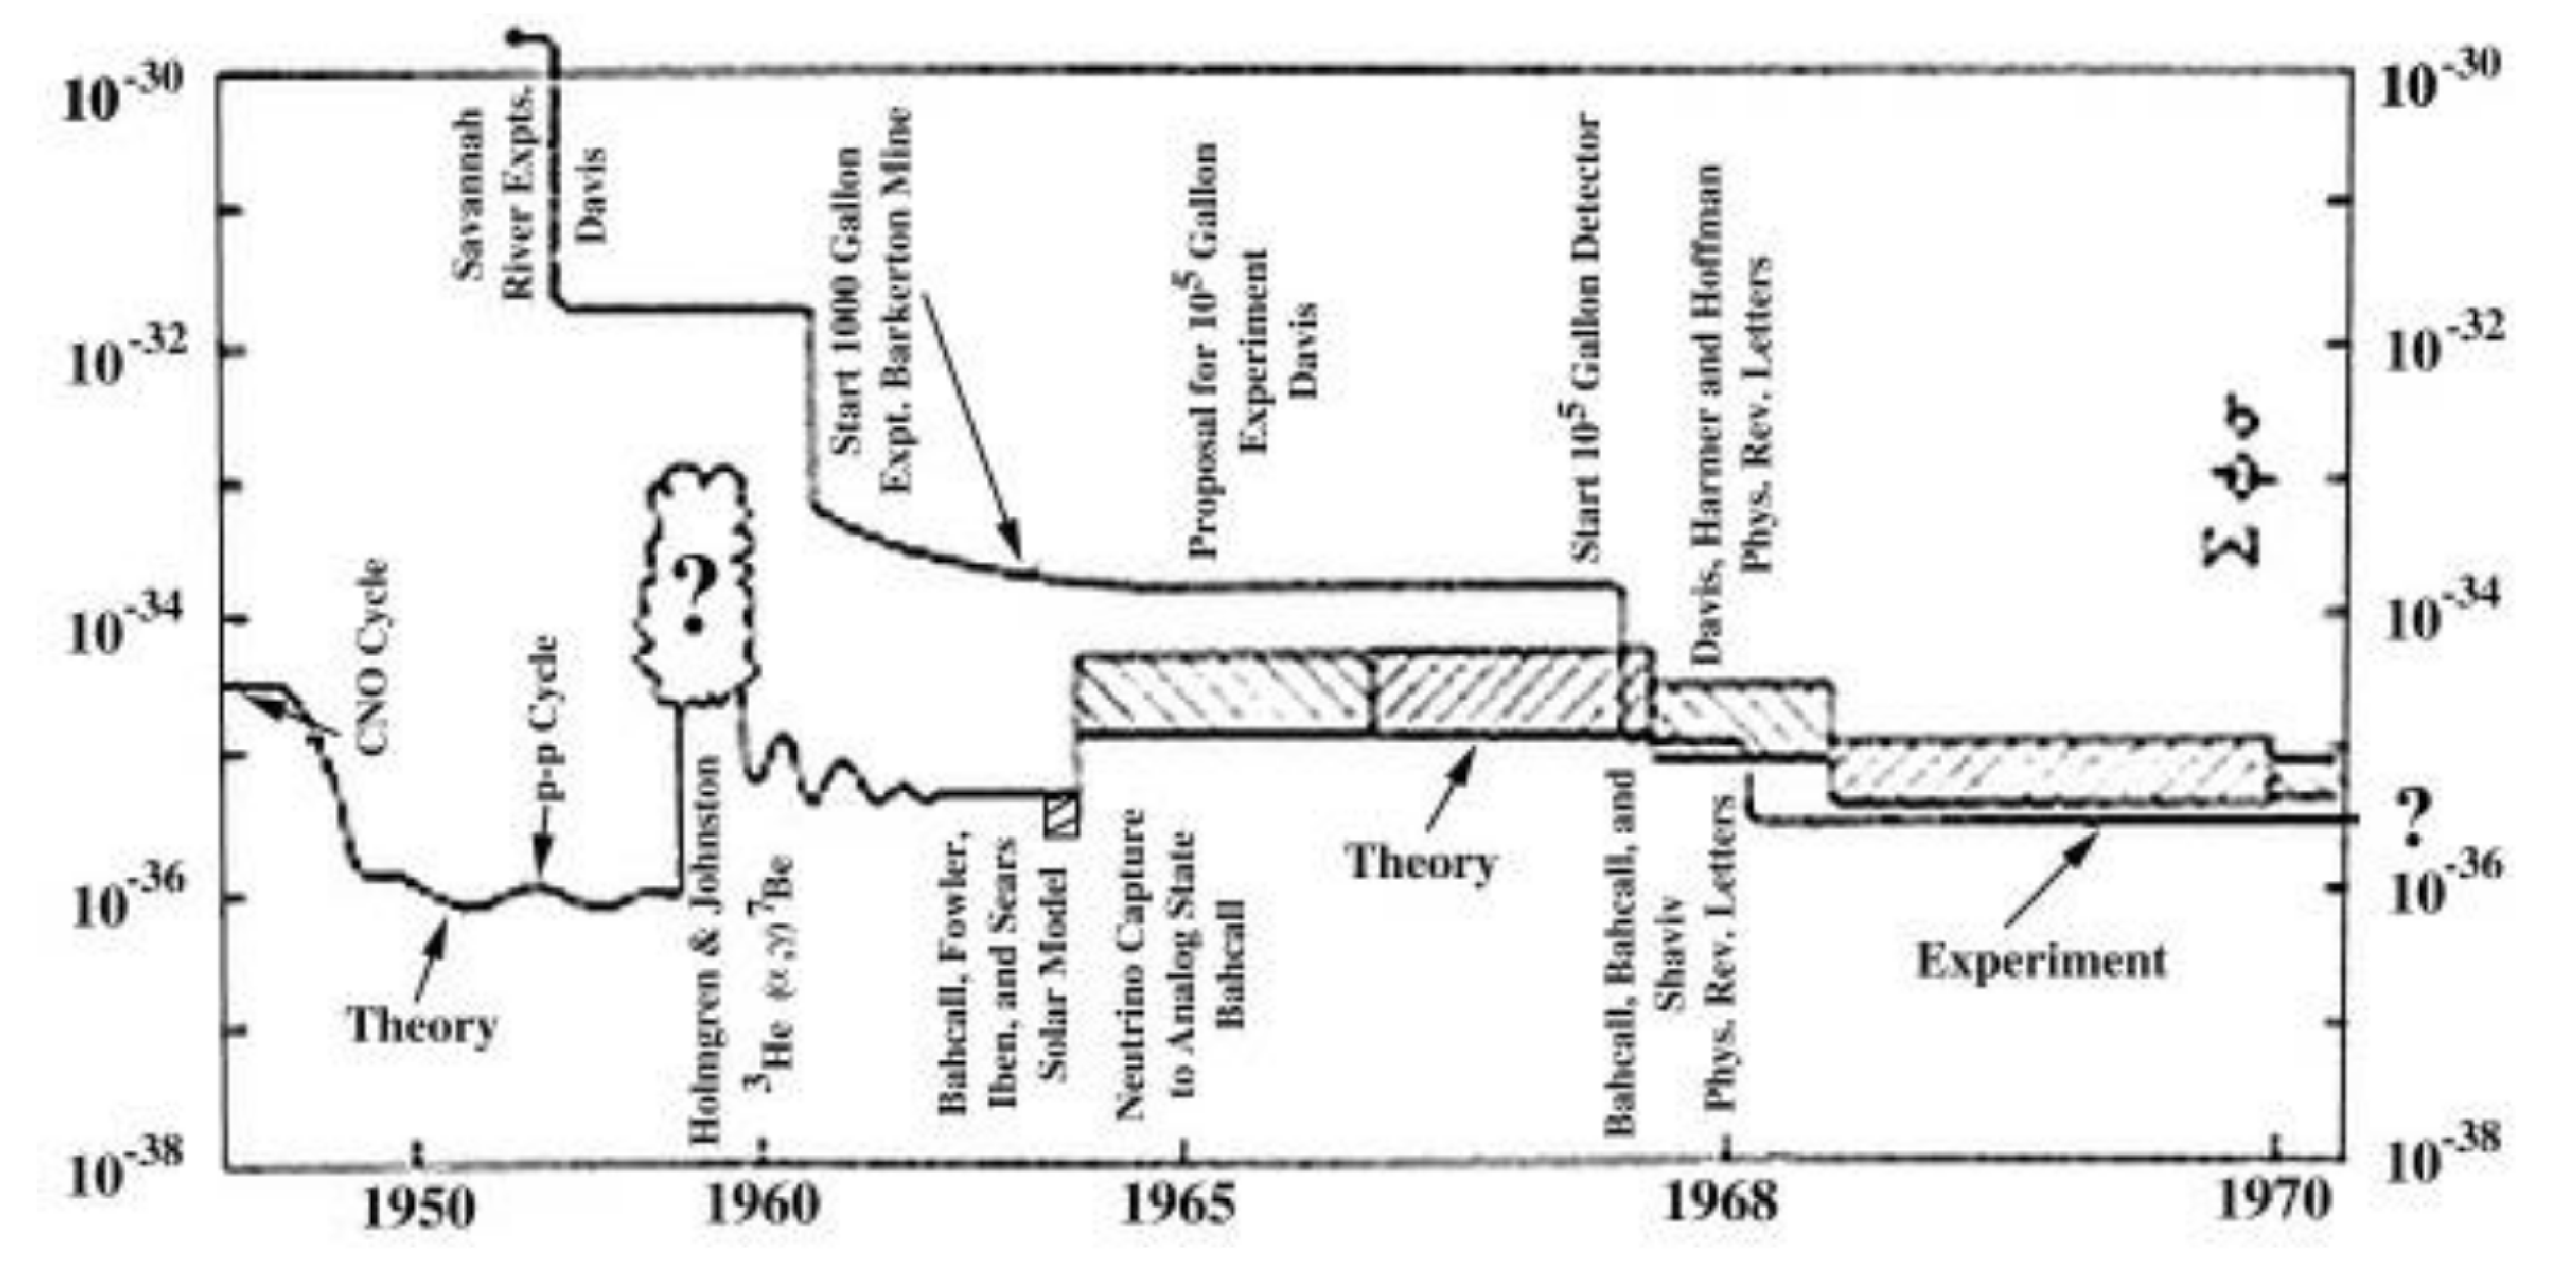
\includegraphics[width=0.75\textwidth]{bahcall_evolution}
\caption[Evolution of Solar Neutrino Predictions and Observations]{
The evolution in the predicted and detectable flux of neutrinos from the sun.
Figure from Ref.~\citep{bahcall_evolution}.}
\label{fig:solar_evolution_cartoon}
\end{figure}

Modern modelling of the Sun and stars could be said to have begun in 1920 with
Arthur Eddington's proposal that nuclear reactions fuel stellar burning~\citep{eddington}.
Bethe's 1938 calculations of solar energy production~\citep{bethe1, bethe2}
followed Eddington's proposal and produced the first model for stellar evolution and burning.
This model was developed over the years as knowledge of nuclear interaction
improved, eventually resulting in Bahcall's comprehensive summary of and
prediction for the Sun's rates of neutrino
production~\citep{bahcall_solar_neutrinos_theory}.
Simultaneous to improvements in solar and nuclear modeling,
particle detection techniques had developed and
the first solar neutrino detector, the Homestake experiment, began
operations in 1967~\citep{homestake_initial}.
The Homestake experiment provided the first experimental measurement
of solar neutrinos and measured a flux that was approximately half what was expected~\citep{homestake}.
Bahcall and Davis~\citep{bahcall_evolution} depicts the evolution in solar neutrino predictions and
the limits of experimental observation with plot shown in Fig.~\ref{fig:solar_evolution_cartoon}.

The persistent deficit observed by the Homestake experiment
eventually became known as the ``Solar Neutrino Problem''.
It was the first evidence that the flavor of neutrinos oscillates with
time, and that therefore neutrinos must have mass.
Conclusive evidence for neutrino oscillation came from  atmospheric neutrino
measurements by the Super Kamiokande and Irvine-Michigan-Brookhaven (IMB)
experiments~\citep{superk_atmospherics, imb_atmospherics}.
And the Solar Neutrino Problem was conclusively resolved by flavor
independent solar neutrino measurement done
by the Sudbury Neutrino Observatory (SNO)~\citep{sno_first, sno_second, solar_nu_problem}.
More will be said about the Super Kamiokande and SNO experiments in
Sec.~\ref{sec:experiments}.

\section{Neutrino Interactions}
\label{sec:neutrino_interactions}
The neutrino interacts almost exclusively via the weak interaction.
In principle neutrinos also interacts gravitationally and they have a non-vanishing
magnetic moment so can interact electromagnetically, but these
interaction potentials are so small they can be neglected in all practical
cases~\citep{neutrino_magmom}.
The weak interaction has a number of aspects that limit the sort of neutrino
interactions that can occur. One aspect is lepton flavor conservation,
all weak interactions conserve both the total lepton number of a system, but also
the total lepton flavor of the system as well.
This leads to nearly all interactions involving a neutrino also involving the
same flavor charged lepton.
The second aspect is that the weak interaction is chiral,
only left-handed particles and right-handed anti-particles interact weakly.
Since neutrinos only interact weakly, the only detectable varieties of neutrino
is the left-handed neutrino $\nu^{L}$  and the right-handed
anti-neutrino $\overline{\nu}^{R}$~\citep{weinberg}.

Discussed here are the neutrino interactions occur in the energy regime
relevant for solar neutrinos.
At higher energies, $E_{\nu} \gtrapprox 100$\,MeV, neutrinos can interact
with nuclear targets through quasi-elastic scattering, resonant
pion-production, or deep inelastic scattering.
A more complete overview of neutrino interactions is available in Ref.~\citep{neutrino_xsec}.

\begin{figure}[htbp]
\centering
\begin{feynman}
\fermion[label=$\overline{\nu}_{e}$]{0.00, 0.00}{1.50, 1.00}
\fermion[label=$p$]{3.00, 0.00}{1.50, 1.00}
\electroweak[label=$W^{+}$]{1.50, 1.00}{1.5, 2.00}
\fermion[label=$e^{+}$]{1.50, 2.00}{0.0, 3.00}
\fermion[label=$n$]{1.5, 2.00}{3.00, 3.00}
\end{feynman}
\caption[Inverse Beta Decay Feynman Diagram]{Feynman diagram for the 
inverse beta decay process.}
\label{fig:ibd}
\end{figure}
At lower energies one of the most common methods for detecting (anti)neutrinos
is through inverse beta-decay (IBD), $\overline{\nu}_{e} + p \rightarrow n + e^{+}$.
Figure~\ref{fig:ibd} shows the Feynman diagram for this process.
The Cowan \& Reines experiment used this interaction to establish the existence
of the neutrino and reactor neutrino experiments still use this interaction as
their primary detection method~\citep{double_chooz1, daya_bay, reno}.
These experiments take advantage of the fact that the IBD positron and neutron
will both interact in their detector, producing a pair
of events with a known, typically very short, time delay.
By looking for pairs of events instead of a single interaction almost
all backgrounds can be removed.

\begin{figure}[htbp]
\centering
\begin{subfigure}[b]{0.48\textwidth}
\begin{feynman}
\fermion[label=$e^{-}$]{0.00, 0.00}{1.00, 1.00}
\fermion[label=$\nu_{e}$]{1.00, 1.00}{0.00, 2.00}
\electroweak[label=$W^{+}$]{1.00, 1.00}{2.0, 1.00}
\fermion[label=$n$]{3.00, 0.00}{2.0, 1.00}
\fermion[label=$p$, showArrow=true]{2.0, 1.00}{3.00, 2.00}
\end{feynman}
\caption[]{}
\label{fig:nuclear_cc}
\end{subfigure}
\hfill
\begin{subfigure}[b]{0.48\textwidth}
\begin{feynman}
\fermion[label=$e^{-}$]{0.00, 0.00}{1.00, 1.00}
\fermion[label=$\nu_{e}$]{1.00, 1.00}{0.00, 2.00}
\electroweak[label=$Z$]{1.00, 1.00}{2.0, 1.00}
    \fermion[label=$p\mathrm{,}n$]{3.00, 0.00}{2.0, 1.00}
    \fermion[label=$p\mathrm{,}n$, showArrow=true]{2.0, 1.00}{3.00, 2.00}
\end{feynman}
\caption[]{}
\label{fig:nuclear_nc}
\end{subfigure}
  \caption[Neutrino Nuclear Interactions]{Charged current (a) and neutral current (b)
  neutrino nuclear interactions.}
\label{fig:nuclear_interactions}
\end{figure}

Also significant at lower energies is the charged current (CC) nuclear interaction
$\nu_{e}$~$+$~$n$~$\rightarrow$~$p$~$+$~$e^{-}$.
Figure~\ref{fig:nuclear_cc} gives the Feynman diagram for this process.
The charged current nuclear interaction played a significant role in early
radio-chemical solar neutrino experiments~\citep{homestake, sage, gallex, gno}.
SNO made use of the charged current nuclear interaction and the similar neutral
current (NC) interaction (Fig~\ref{fig:nuclear_nc}).
SNO and its measurements will be discussed in greater detail in Sec~\ref{sec:sno}.

\label{sec:esxsec}
% ES diagrams
\begin{figure}
\centering
\begin{subfigure}[t]{0.48\textwidth}
\centering
\begin{feynman}
\fermion[label=$e^{-}$]{0.00, 0.00}{0.80, 0.80}
\fermion[label=$\nu_{e}$]{0.80, 0.80}{0.00, 1.60}
\electroweak[label=$W^{+}$]{0.80, 0.80}{2.0, 0.80}
\fermion[label=$\nu_{e}$]{2.80, 0.00}{2.0, 0.80}
\fermion[label=$e^{-}$, showArrow=true]{2.0, 0.80}{2.80, 1.60}
\end{feynman}
\caption[Charged Current Elastic Scattering Feynman Diagram]{
Charged current elastic scattering interaction}
\label{fig:ES_CC}
\end{subfigure}
\hfill
\begin{subfigure}[t]{0.48\textwidth}
\centering
\begin{feynman}
\fermion[label=$\nu_{x}$]{0.00, 0.00}{0.80, 0.80}
\fermion[label=$\nu_{x}$]{0.80, 0.80}{0.00, 1.60}
\electroweak[label=$Z$]{0.80, 0.80}{2.0, 0.80}
\fermion[label=$e^{-}$, flip=true]{2.00, 0.80}{2.8, 0.00}
\fermion[label=$e^{-}$, showArrow=true ]{2.0, 0.80}{2.80, 1.60}
\end{feynman}
\caption[Neutral Current Elastic Scattering Feynman Diagram]{
Neutral current elastic scattering interaction}
\label{fig:ES_NC}
\end{subfigure}
\label{fig:feynman_es}
\caption[Elastic Scattering Feynman Diagrams]{The Feynman diagrams for the
    charged current elastic scattering interaction\,(a) and the neutral
    current elastic scattering interaction\,(b).}
\end{figure}

Neutrino-electron elastic scattering (ES) is an important neutrino interaction
channel for this work --- it is the main interaction through which neutrinos are
detected in Chapter~\ref{sec:sigex}.
The ES process is $\nu_{\mathrm{x}} + e^{-} \rightarrow \nu_{\mathrm{x}} +e^{-}$
or $\overline{\nu}_{\mathrm{x}} + e^{-} \rightarrow \overline{\nu}_{\mathrm{x}} +e^{-}$.
The tree level Feynman diagrams for the charged current neutrino elastic scattering
interaction is shown in Fig.~\ref{fig:ES_CC} and the neutral current elastic
scattering interaction in Fig.~\ref{fig:ES_NC}.
The neutral current interaction involves $\nu_{\mathrm{x}}$ where $x=\mathrm{e, \mu, \tau}$,
and the charged current interaction involves only $\nu_{\mathrm{e}}$.

The charged current interaction is in principle available to neutrinos of all
flavors, however, for solar neutrinos only the electron flavor version of the
interaction is available.
The initial electron on the left hand side of the interaction is usually understood to
be from an atom within target the detector, and therefore at rest within
the lab frame.
So the total energy in the interaction is simply $E = E_{\nu} + m_{e}$.
For even the highest energy solar neutrinos $E<20$\,MeV, far less that muon
rest mass of $m_{\mu}=105.7$\,MeV/$\text{c}^{2}$ or tau mass $m_\tau = 1776.8$\,MeV/$\text{c}^{2}$.
Meaning a muon or tau cannot be created; the electron with a rest mass
of $m_{e}=0.511$\,MeV/$\text{c}^{2}$ is the only charged lepton that can
be created from the CC-ES interaction for solar neutrinos.
And since lepton flavor is conserved in weak interactions, the electron neutrino
is the only neutrino that can produce an electron, therefore the electron
neutrino is the only neutrino flavor that can undergo the charged-current
elastic scattering interaction.


This flavor disparity in the interaction means that the cross-section for the
elastic scattering process is larger for $\nu_{e}$ than it is for a $\nu_\mu$
or $\nu_\tau$, and the cross-section for a $\nu_\mu$ is the same as that for a
$\nu_\tau$.
The differential cross section of for the diagrams shown in Fig~\ref{fig:ES_CC} and
Fig.~\ref{fig:ES_NC} can be calculated as
\begin{equation}
    \frac{d\sigma}{dT_{\mathrm{e}}}\left(E_{\nu}\text{, }T_{\mathrm{e}}\right)=
    \frac{\sigma_{0}}{m_{\mathrm{e}}}\left[g_{1}^{2} + g_{2}^{2}\left(1 - \frac{T_{\mathrm{e}}}{E_{\nu}}\right)^{2} -g_{1}g_{2}\frac{m_{\mathrm{e}}T_{\mathrm{e}}}{E_{\nu}^{2}}\right]\text{,}
\end{equation}
where,
\begin{equation}
    \sigma_{0} = \frac{2G^{2}_{\mathrm{F}}m_{\mathrm{e}}^{2}}{\pi}\text{.}
\end{equation}
For $\nu_{x} = \nu_{e}$
\begin{equation}
    g_{1} = \frac{1}{2} + \sin^{2}\theta_{\mathrm{W}}\text{,}
\end{equation}
and
\begin{equation}
    g_{2} = \sin^{2}\theta_{\mathrm{W}}\text{.}
\end{equation}
For $\nu_{x} = \nu_{\mu}$ or $\nu_{x} = \nu_{\tau}$ $g_{1}$ and $g_{2}$ are
given by,
\begin{equation}
    g_{1} = \sin^{2}\theta_{\mathrm{W}} - \frac{1}{2}\text{,}
\end{equation}
\begin{equation}
    g_{2} = \sin^{2}\theta_{\mathrm{W}}\text{.}
\end{equation}

Since the electron scattering is elastic, the kinematics of the interaction
leave only one free parameter, the outgoing electron direction with respect
to the incoming neutrino direction, $\theta$.
For a recoil electron with a given value for $\theta$ the electron kinetic energy is
given by
\begin{equation}
    T_{\mathrm{e}}=\frac{2m_{\mathrm{e}}E_{\nu}^{2}\cos^{2}\theta}{(m_{\mathrm{e}}+E_{\nu})^2 - E_{\nu}^{2}\cos^2\theta}\text{.}
    \label{eqn:es_te_theta}
\end{equation}
This relationship can be used to produce the differential cross-section in $\cos\theta$,
\begin{multline}
\frac{d\sigma}{d\cos\theta}=\sigma_{0}\frac{4E_{\nu}^{2}(m_{\mathrm{e}}+E_{\nu}^{2})^2\cos\theta}{\left[(m_{\mathrm{e}}+E_{\nu}^{2} -E_{\nu}^{2}\cos^2\theta)\right]^2}\\
    \left[g_{1}^{2} + g_{2}^{2}\left(1 - \frac{2m_{\mathrm{e}E_{\nu}\cos^{2}\theta}}{(m_{\mathrm{e}}+E_{\nu})^2 -E_{\nu}^{2}\cos^2\theta} \right)^{2} - g_{1}g_{2}\frac{2m_{\mathrm{e}^{2}}\cos^{2}\theta}{(m_{\mathrm{e}}+E_{\nu})^{2}-E_{\nu}^{2}\cos^{2}\theta}\right]
    \text{.}
\end{multline}
And finally the maximum energy a recoil electron will have can be found by
setting $\cos\theta=1$ in equation~\eqref{eqn:es_te_theta}, this yields
\begin{equation}
    T_{e}^{\max}(E_\nu) = \frac{2E_{\nu}^{2}}{m_{\mathrm{e}}+ 2E_{\nu}^{2} }\text{.}
\end{equation}
These results are derived from first princibles in Ref.~\citep{giuntikim}.

\begin{figure}[htbp]
\centering
\begin{subfigure}[b]{0.57\textwidth}
\centering
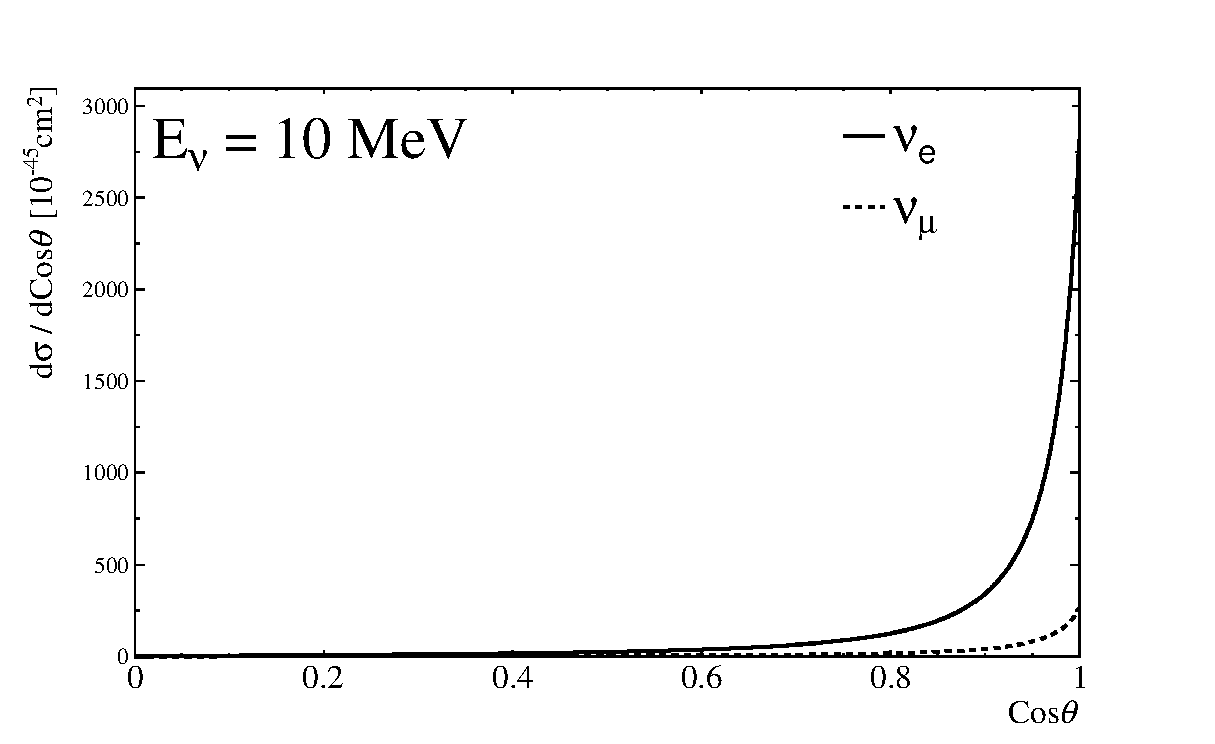
\includegraphics[width=\textwidth]{neutrino_xsec_energy}
\caption[ES Recoil Energy Cross-Section]{}
\label{}
\end{subfigure}
\hfill
\begin{subfigure}[b]{0.57\textwidth}
\centering
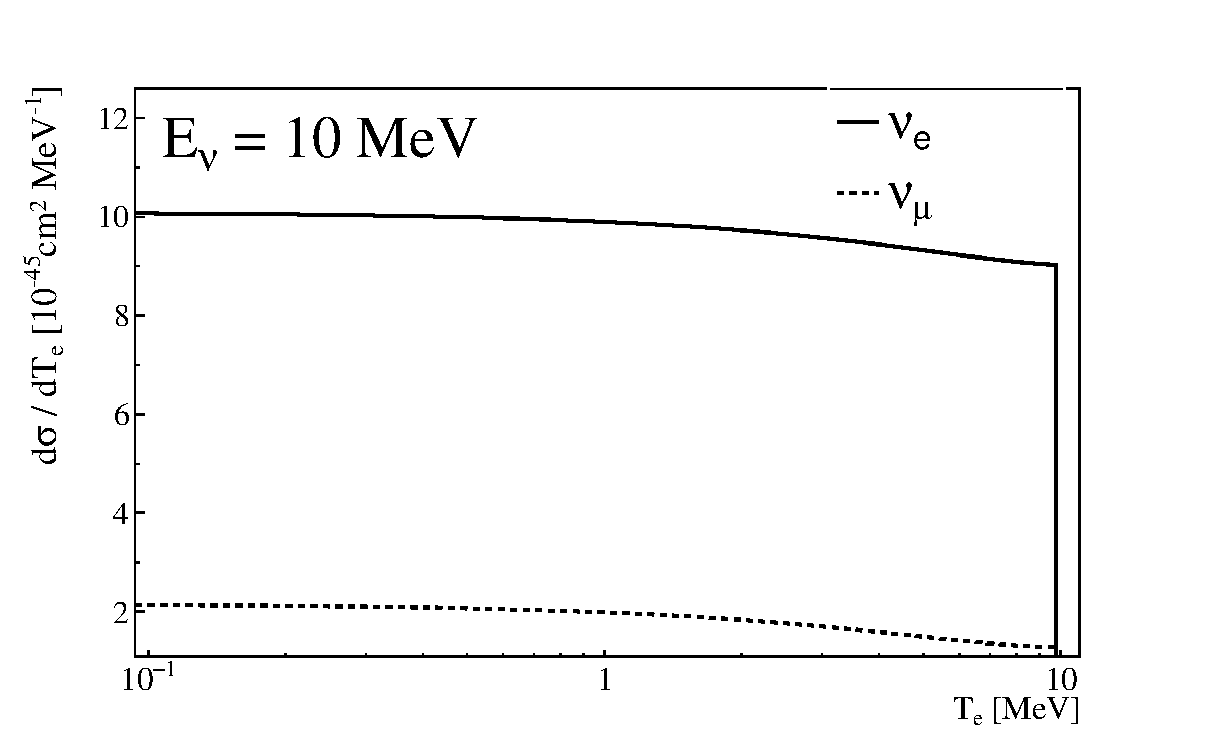
\includegraphics[width=\textwidth]{neutrino_xsec_angular}
\caption[ES Angular Cross-Section]{}
\label{}
\end{subfigure}
\caption[Neutrino-Electron ES Cross-Sections]{The electron recoil\,(a)
cross-section and electron angular\,(b) cross-section for neutrino-electron
elastic scattering with a 10\,MeV incoming neutrino energy.}
\label{fig:es_xsec}
\end{figure}


Figure~\ref{fig:es_xsec} shows the differential cross-sections for a 10\,MeV neutrino.
The fact that the scattering cross-section is peaked near $\cos\theta=1$
is very useufl for neutrino experiments; the observed electron direction
will almost always be nearly co-linear with the incoming neutrino direction.
Unforunately, since the cross-section is nearly flat in $T_{\mathrm{e}}$
the electron energy provides almost no information about the incoming neutrino
energy.
The kinematics and cross-section of the out-going neutrino is also
well predicted with respect to $\cos\theta$, however the out-going
neutrino is typically of little interest because it cannot be detected.

Experimentally neutrino elastic scattering has been studied in a number
of venues historically and recently~\citep{reines2, es_measurement, nutev}.
Famously the first experimental evidence for the $Z$ boson came from
the observations of neutrino elastic scattering at the
Gargamelle experiment~\citep{gargamelle}.
It's also been a useful detection method for water-cherenkov solar
neutrino experiments because the directionality of the interaction
allow events that originate from the Sun to be identified~\citep{sno_first,
kamiokande, superk_first_solar}.

\section{Neutrino Oscillations}
\label{sec:neut_osc}
Neutrino oscillation is a phenomena of massive neutrinos, and it's observation
is currently the only experimental evidence that neutrinos do indeed have mass.
Neutrino oscillation results from the fact that neutrino flavors do not have
well defined masses, instead neutrino flavor states are a quantum superposition
of neutrino mass states.
And conversely, mass states can be described as a superposition of flavor states.
Stated more precisely,
\begin{equation}
    \ket{\nu_{i}} = U_{i\ell}\ket{\nu_\ell}
\end{equation}
Where $\ket{\nu_\ell}$ represents the neutrino flavor states, $\ket{\nu_i}$
represents the mass states, and $U_{i\ell}$ describes the mixing of these
states.
$U$ is known as the Pontecorvo-Maki-Nakagawa-Sakata (PMNS) matrix,
and it is exactly analogous to the Cabibbo-Kobayashi-Maskawa (CKM) matrix used
to describe quark mixing.
In the simplest case where the weak states and the mass states are the same
$U$ would just be the identity matrix.
Under the assumption that there are three flavor states and three mass states
$U_{i\ell}$ must be unitary so that the probability of observing
a neutrino in any state is never less than one.
It is known from observations of Z boson decay products that
there are only three ``active'' neutrino flavors~\citep{Zdecay}.
Where active means that the neutrino participates in
weak interactions.
It's possible there there is a neutrino that does not interact
weakly, this is referred to as a sterile neutrino and is the
subject of a number of experimental searches~\citep{prospect, lsnd, miniboone, jsns2}.
If there were a sterile neutrino state the $3\times3$ PMNS matrix would
no longer be unitary.

It is typical to characterize $U$ with three angles
($\theta_{12}$, $\theta_{13}$, $\theta_{23}$) and a CP violating
phase $\delta_{cp}$. Doing so allows for the general SU(3) mixing matrix to
be decomposed into two SO(2) matrices and one SU(2) matrix,
$$U_{12} =
\begin{bmatrix}
    \cos\theta_{12} & \sin\theta_{12} & 0  \\
    -\sin\theta_{12}& \cos\theta_{12} & 0  \\
    0 & 0 & 0  \\
\end{bmatrix},
$$
$$
U_{13} =
\begin{bmatrix}
    \cos\theta_{13} & 0 & \sin\theta_{13}e^{-i\delta_{cp}}\\
    0 & 0 & 0  \\
    -\sin\theta_{13} e^{-i\delta_{cp}} & 0 & \cos\theta_{13}  \\
\end{bmatrix},
$$
$$
U_{23} =
\begin{bmatrix}
    0 & 0 & 0  \\
    0 & \cos\theta_{23} & \sin\theta_{23} \\
    0 & -\sin\theta_{23} & \cos\theta_{23}   \\
\end{bmatrix}.
$$
The product of these matrices produces the full mixing matrix,
$U = U_{23}U_{13}U_{12}$.

The mixed nature of neutrino flavor and mass states gives rise to oscillations
in the flavor content of propagating neutrinos.
By definition the neutrino mass states are eigenstates of the vacuum Hamiltonian
\begin{equation}
    H\ket{\nu_{i}} = E_{i}\ket{\nu_{i}}\text{,}
\end{equation}
where the energy is given by the standard relativistic energy equation,
\begin{equation}
    E_{i} = \sqrt{{(p_{i}c)}^{2} + {(m_{i}c^{2})}^2}\text{.}
\end{equation}
It is typical to make the assumption that all neutrino mass states have the same
momentum, $p_{i} = p$.
The equal momentum assumption allows for a straightforward derivation of the
correct description of neutrino oscillations, but it is not well motivated.
A discussion of the equal momentum assumption and its validity
is available in Ref~\citep{neutrino_osc_subtleties}.

Applying Schrodinger's equation,
\begin{equation}
    i\frac{d}{dt}\ket{\nu_{i}(t)} = H\ket{\nu_{i}(t)} = E_{i}\ket{\nu_{i}(t)}\text{,}
\label{eq:mass_state_evolution}
\end{equation}
results in,
\begin{equation}
    \ket{\nu_{i}(t)} = e^{-iE_{i}t}\ket{\nu_{i}(t=0)}\text{.}
    \label{eqn:mass_state_tevol}
\end{equation}

This time evolution of mass eigenstates can be used to then describe the state
of a neutrino that is created in a electron flavor eigenstate.
\begin{equation}
\ket{\nu(t=0)} = \ket{\nu_{e}} = U_{1e}\ket{\nu_1} + U_{2e}\ket{\nu_{2}} + U_{3e}\ket{\nu_{3}}
    =\sum_{i=1}^{3}U_{ie}\ket{\nu_{i}}
\end{equation}

Each of the mass states' time evolution can be immediately written down from
Equation~\eqref{eqn:mass_state_tevol},
\begin{equation}
    \ket{\nu(t)} = \sum_{i=1}^{3} U_{ie}e^{-iE_{i}t}\ket{\nu_{i}}\text{.}
    \label{eqn:e_state}
\end{equation}

From Eqn.~\eqref{eqn:e_state} the quantity that's often of the most interest
is the survival probability, defined as
\begin{equation}
    P_{ee}(t) = \abs{\braket{\nu_{e}}{\nu(t)}}^{2}\text{.}
\end{equation}
$P_{ee}(t)$ can be understood as the probability that a neutrino, produced in
an electron flavor state, will be detected as an electron flavor state a time
$t$ later.
The survival probability for the state given in Eqn.~\eqref{eqn:e_state} is
\begin{equation}
    P_{ee}(t) = \sum_{i,j}\abs{U_{ei}}^2\abs{U_{ej}}^2e^{-i(E_{i} - E_{j})t}\text{.}
\end{equation}
It is useful to separate out the terms where $i=j$,
\begin{equation}
    P_{ee}(t) = \sum_{i}\abs{U_{ei}}^4 + \sum_{i,j\text{, }j \ne i}
    \abs{U_{ei}}^2\abs{U_{ej}}^2e^{-i(E_{i} - E_{j})t}\text{.}
\end{equation}
Here we can see there are terms that vary with time, and terms that are
constant.

A few more simplifications are commonly done, using the equal momentum
assumption mentioned earlier and the fact the neutrino rest mass is
very small, the energy differences can be simplified,
\begin{equation}
    E_{i} - E_{j} = \sqrt{p^{2} + m_{i}^{2}} - \sqrt{p^{2} + m_{j}^{2}} \approx
    p^{2} - p^{2} + \frac{m_{i}^2}{2p} - \frac{m_{j}^2}{2p}\text{.}
\end{equation}
To good approximation $p^2=E^2$, so
\begin{equation}
    E_{i} - E_{j} = \frac{\Delta m^{2}_{ij}}{2E}\text{,}
\end{equation}
where the definition of the mass-squared splittings is used,
\begin{equation}
    \Delta m^{2}_{ij} = m^{2}_{i} - m^{2}_{j}\text{.}
\end{equation}

The final simplification is to assume that the neutrino is moving very close
to the speed of light, therefore any flavor oscillations over time will also
occur at a distance $L$ from the neutrino's creation.
All this gives
\begin{equation}
    \label{eqn:pee_adiabatic}
    P_{ee}(L,E) = \sum_{i}^{3}\abs{U_{ei}}^4 +
    \sum_{i,j\text{, }j \ne i}^{3}
    \abs{U_{ei}}^2\abs{U_{ej}}^2e^{-i\left(\frac{\Delta m^{2}_{ij}}{2E}L\right)}\text{.}
\end{equation}
For the mixing parameters given in~\citep{PDG2016} the average survival probability
for a electron neutrino is $P_{ee} = 55.8\%$.

It's common to represent neutrino mixing in the following form
\begin{equation}
i\frac{d}{dt}\ket{\Psi_{\alpha}} = H\ket{\Psi} = \frac{1}{2E}UM^{2}U^{\dagger}\ket{\Psi_{\alpha}}\text{.}
\label{eq:mixing_hamiltonian}
\end{equation}
Where $U$ is the PMNS matrix, $\Psi_{\alpha}$ is the neutrino state in the  flavor
basis, and
\begin{equation}
M^{2} = 
\begin{bmatrix}
    0 & 0 & 0  \\
    0 & \Delta m^{2}_{21} & 0  \\
    0 & 0 & \Delta m^{2}_{31}  \\
\end{bmatrix}\text{.}
\end{equation}
This form of the mixing equation is the same as Eqn.~\eqref{eq:mass_state_evolution}
written in the flavor basis.


With the exception of the CP violating phase $\delta_{cp}$, all mixing
parameters and mass-squared splitting have been measured experimentally~\citep{pdg_globalfit}.
None of the parameters are predicted in the standard model, so they are theoretically
unconstrained.
The measurements of the mass-squared splittings and
other parameters are discussed in Sec.~\ref{sec:experiments}.
The absolute mass of each neutrino state is not yet known.
There are upper limits placed on the sum of the neutrino masses from
observations of tritium decay~\citep{troitsk_mass}, and from cosmological
observations and modelling~\citep{cosmological_neutrino_mass}.

Also unknown is the ``hierarchy'' of the neutrino masses, i.e.\ which
mass states are heavier or lighter than the others.
Solar neutrino measurements have established that the $\nu_{2}$ state
is more massive than the $\nu_{1}$ state~\citep{sno_first, sno_combined}, but so far no experiment has been
able to resolve if $\nu_{3}$ is more or less massive than $\nu_{1}$ and $\nu_{2}$ states~\citep{vogel_hierarchy}.
The case where the $\nu_{1}$ state is the lightest is referred to as the
``normal hierarchy'' because then neutrino mass state have the same
ordering as the charged leptons;
the case where $\nu_{3}$ is the least massive neutrino is known as the
 ``inverted hierarchy'', because then the neutrino mass states are opposite
 that of the charged lepton states.
 Experimental measurements and cosmological consdierations currently prefer
 the normal hierarchy over the inverted hierarchy at approximately $2.4\sigma$ statistical
 significance~\citep{nu_fit}

The model of neutrino mixing as described assumes that neutrinos are Dirac, as opposed to
Majorana. In the case that the neutrino is a Majorana particle the PMNS matrix
gains two additional complex ``Majorana'' phases, similar to the CP violating
phase $\delta_{CP}$.
However, neutrino oscillation observables, such as the survival and transition
probability, are in general not effected by the Majorana phase~\citep{majorana_mixing}.
Therefore it is accurate to ignore the presence of Majorana phases in typical 
neutrino mixing calculations regardless of the true Majorana or Dirac nature of the neutrino.

\subsection{Matter Enhanced Oscillations}
When neutrinos propagate through matter, as opposed to vacuum, its oscillation is altered
by the potential introduced from available nuclear and leptonic interactions.
The interaction comes primarily from a neutral current interaction of the form
shown in Fig.~\ref{fig:nuclear_nc}, and a flavor dependent charged current interaction shown in
Fig.~\ref{fig:nuclear_cc} and the  neutrino-electron elastic scattering interaction shown in
Fig.~\ref{fig:ES_CC} and Fig.~\ref{fig:ES_NC}.
The potential for the nuclear charged current interaction is negligible
because it modifies the state of the nucleon it interacts with,
and is thus considered an incoherent nuclear interaction.
It is shown in Ref.~\citep{wolfenstein_osc} that incoherent interactions
will contribute negligibly to the interaction potential except if the neutrinos
are extremely high energy or in regions of extremely high matter density.

The potential energy associated with the charged current ES interaction
is given by
\begin{equation}
V_{\mathrm{CC}} = \sqrt{2}G_{F}N_{\text{e}}\text{,}
\end{equation}
where $N_{\mathrm{e}}$ is the local electron density.
Similarly the neutral current interactions contribute a flavor independent
shift to the potential given by
\begin{equation}
V_{\mathrm{NC}} = -\frac{\sqrt{2}}{2} G_{\text{F}} N_{\mathrm{n}}
\end{equation}
where $N_{n}$ is the local neutron density, the contributions to this potential
from electron and proton interactions cancel out.
This derivation assumes the neutrino is traveling through matter composed primarily
of protons, neutrons, and electrons.
 A safe assumption for almost all cases.

The mixing described by Eqn.~\eqref{eq:mixing_hamiltonian} is modified to include
the potential terms described above.
\begin{equation}
i\frac{d}{dt}\ket{\Psi_{\alpha}} = \left[H_{\mathrm{vac}} + H_{\mathrm{I}}\right]\ket{\Psi}
\end{equation}
\begin{equation}
H_{\mathrm{vac}}  = \frac{1}{2E}UM^{2}U^{\dagger}
\end{equation}
\begin{equation}
 H_{\mathrm{I}} =  A_{\mathrm{CC}} + A_{\mathrm{NC}}\text{.}
\end{equation}
The mixing potentials for the charged and neutral current interactions
are given by
\begin{equation}
A_{\mathrm{CC}} = 
\begin{bmatrix}
    V_{\mathrm{CC}} & 0 & 0  \\
    0 & 0 & 0  \\
    0 & 0 & 0\\
\end{bmatrix}\text{,}
\end{equation}
\begin{equation}
A_{\mathrm{NC}} = 
\begin{bmatrix}
    V_{\mathrm{NC}} & 0 & 0  \\
    0 & V_{\mathrm{NC}} & 0  \\
    0 & 0 & V_{\mathrm{NC}}\\
\end{bmatrix}\text{.}
\end{equation}
It can be show that since $A_{\mathrm{NC}}$ is identity-like it can be neglected
from consideration;
identity-like matrices produce no observable effect on the overall neutrino mixing.
The full mixing Hamiltonian is given by
\begin{equation}
H = \frac{1}{2E}UM^{2}U^{\dagger} + A_{\mathrm{CC}}\text{.}
\end{equation}
These results are derived in detail in Ref.~\cite{wolfenstein_osc} and Ref.~\citep{giuntikim}.

It's clear that the electron density through which a
neutrino propagates can modify the effective mass-splitting and mixing angle
for the electron neutrino.
That is to say, any matter-enhanced mixing can also be described as vacuum mixing
with just a different set of mixing parameters.
For a given neutrino energy $E_{\nu}$ there exists an electron density for which
the effective mixing angle is maximal, this is known as the resonant density~\citep{wolfenstein_osc, ms_oscillation}.
This resonance is important for solar neutrinos and will be discussed further in
the next section.

Matter effects also introduce the question of adiabaticity into neutrino
oscillations.
As a neutrino travels through changing matter potentials its possible for
the effective potential to evolve much faster than the neutrino oscillates.
A neutrino's propagation is said to be fully adiabatic if its mass state composition
does not change between production and detection.
A specific example is if a neutrino state is a pure vacuum mass-1
state,
\begin{equation*}
    \ket{\Psi_{\nu}} = \ket{\nu_{1}}
\end{equation*}
suddenly enters a region of significant electron density where the mass states
are now $\ket{\nu_{k}^\prime}$.
The neutrino state does not have time to evolve at all so the state
does not change, but it is not longer a pure eigenstate of the mixing
Hamiltonian,
\begin{equation*}
    \ket{\Psi_{\nu}} = \ket{\nu_{1}} = \sum_{k=1}^{3} \braket{\nu_{k}^\prime}{\nu_{1}}\ket{\nu_{k}^\prime}\text{.}
\end{equation*}
Since the neutrino is no longer in a pure eigenstate the state will
now oscillate.

In contrast if the neutrino enters the region of significant electron
density more slowly, then the neutrino state will smoothly evolve with the
eigenstate, $\ket{\nu_{1}} \rightarrow \ket{\nu_{1}^{\prime}}$.
And so the final state of the neutrino in the adiabatic case will be,
\begin{equation*}
    \ket{\Psi_{\nu}} = \ket{\nu_{1}^{\prime}}\text{.}
\end{equation*}

%The adiabaticity of neutrino evolution will be discussed further in Chapter~\ref{sec:chameleons}.

\section{Solar Neutrinos}
\begin{figure}[htbp]
\centering
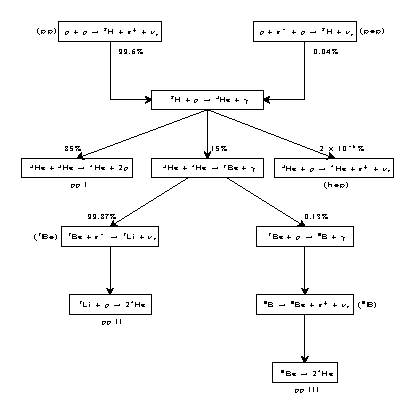
\includegraphics[width=0.8\textwidth]{pp_chain}
\caption[$pp$ Chain Solar Reactions]{The $pp$ chain reactions with
branching ratios for the Sun, values from~\citep{bahcall_book}.}
\label{fig:pp_chain}
\end{figure}
\begin{figure}[htbp]
\centering
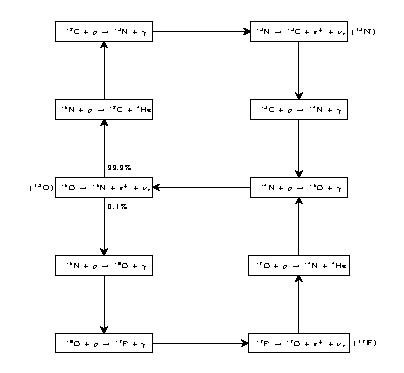
\includegraphics[width=0.8\textwidth]{cno_cycle}
\caption[CNO Cycle Solar Reactions]{The CNO cycle reactions with
branching ratios for the Sun, values from~\citep{bahcall_book}.}
\label{fig:cno_cycle}
\end{figure}
Nuclear reactions in the core of the Sun provides the main fuel for
stellar burning and prevents the Sun from collapsing due to gravitation
pressure.
There exists two separate chains of nuclear reactions that are present in typical
stellar conditions, the $pp$-chain and the CNO-cycle~\citep{bahcall_solar_neutrinos_theory}.
Figure~\ref{fig:pp_chain} and~\ref{fig:cno_cycle} shows these two reaction chains.
For the Sun the $pp$ chain
provides 99\% of the generated nuclear energy, and the CNO-cycle provides the remaining
1\%. For stars significantly more massive than the Sun, the CNO-cycle is the
main energy generating mechanism.
%The CNO-cycle has the interesting property of conserving the atmoic abundance of the atomic

\begin{figure}[htbp]
\centering
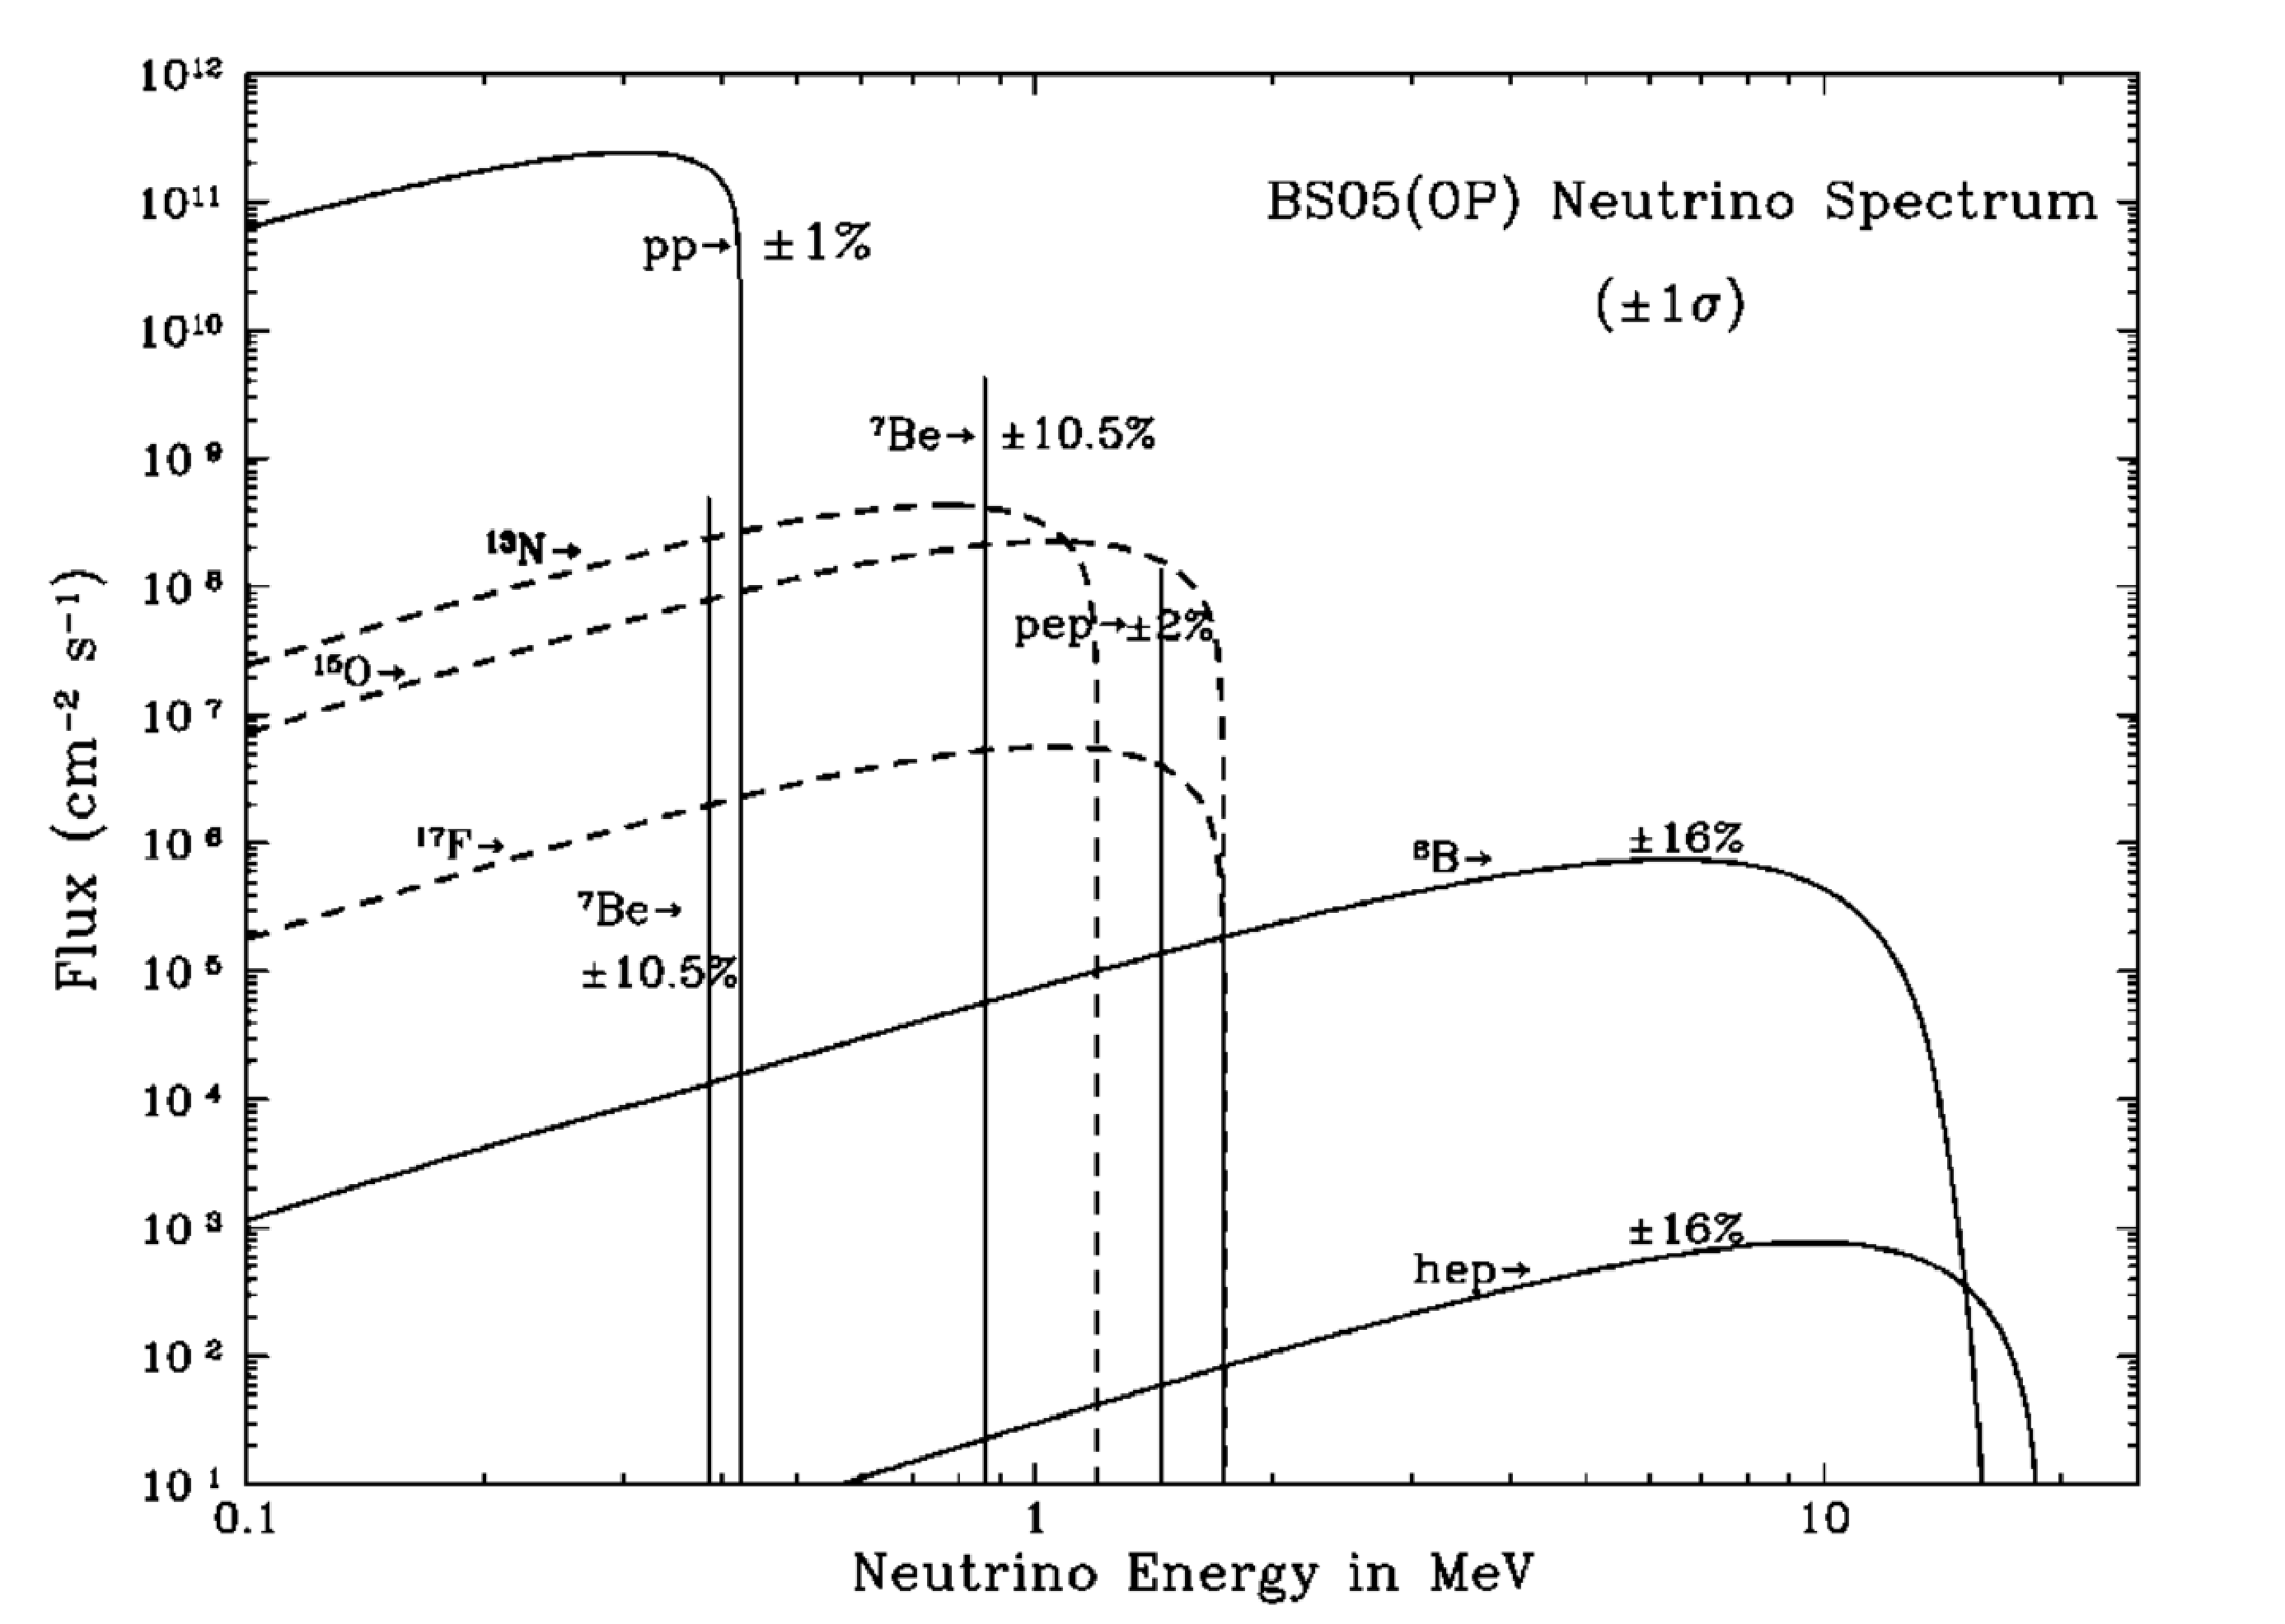
\includegraphics[width=0.6\textwidth]{bs05op_spectrum}
\caption[Solar Neutrino Spectrum]{Energy spectrum for neutrinos from
the Sun with normalization uncertainties. Figure from~\citep{bs_ssm}.}
\label{fig:bs05_spectrum}
\end{figure}

Within the $pp$-chain there are five processes that produce neutrinos.
Since the Q-value of the processes in the $pp$ chain are all below the rest mass
of a muon or tau, the only charged lepton generated is electrons. And so from
lepton flavor conservation only electron flavor neutrinos are generated.
And because the neutrino producing processes are all fusion reactions or
$\beta^{+}$ decay, only neutrinos are produced and not any anti-neutrinos.
Neutrinos are produced with an energy spectrum shown in Fig.~\ref{fig:bs05_spectrum}.

The $hep$ and $\ce{^{8}B}$ reactions produce neutrinos with the highest
energies. Since the $hep$ reaction branching ratio is so low the flux
of $hep$ neutrinos is also very low compared to that of $\ce{^{8}B}$ neutrinos;
the $hep$ flux is expected to be approximately $0.15\%$ of the $\ce{^{8}B}$ flux.
So for water-Cherenkov detectors that have a typical threshold of a few MeV,
$\ce{^{8}B}$ neutrinos are the primary source of detectable solar neutrinos.
The uncertainty on the predicted $\ce{^{8}B}$ flux is relatively large, this comes mostly
from the uncertainty on the cross-sections and how those cross-sections change with
temperature, and uncertainties on the temperature profile within the core of the Sun.
And because the $\ce{^{8}B}$ reaction has five preceding reactions the uncertainty on
 those reactions are part of the uncertainty on the $\ce{^{8}B}$ flux~\citep{bs_ssm}.

The uncertainty on the $pp$ and $pep$ neutrinos is much lower for two reasons. First, because
they are at early stage of the reaction chain, so their reaction rate is not dependent on any
other preceding interaction. The $pp$ reaction is also the main energy generating mechanism
for the Sun, so measurements of the total solar luminosity provide strict constraints on the
$pp$ flux as well.

\begin{figure}[htbp]
\centering
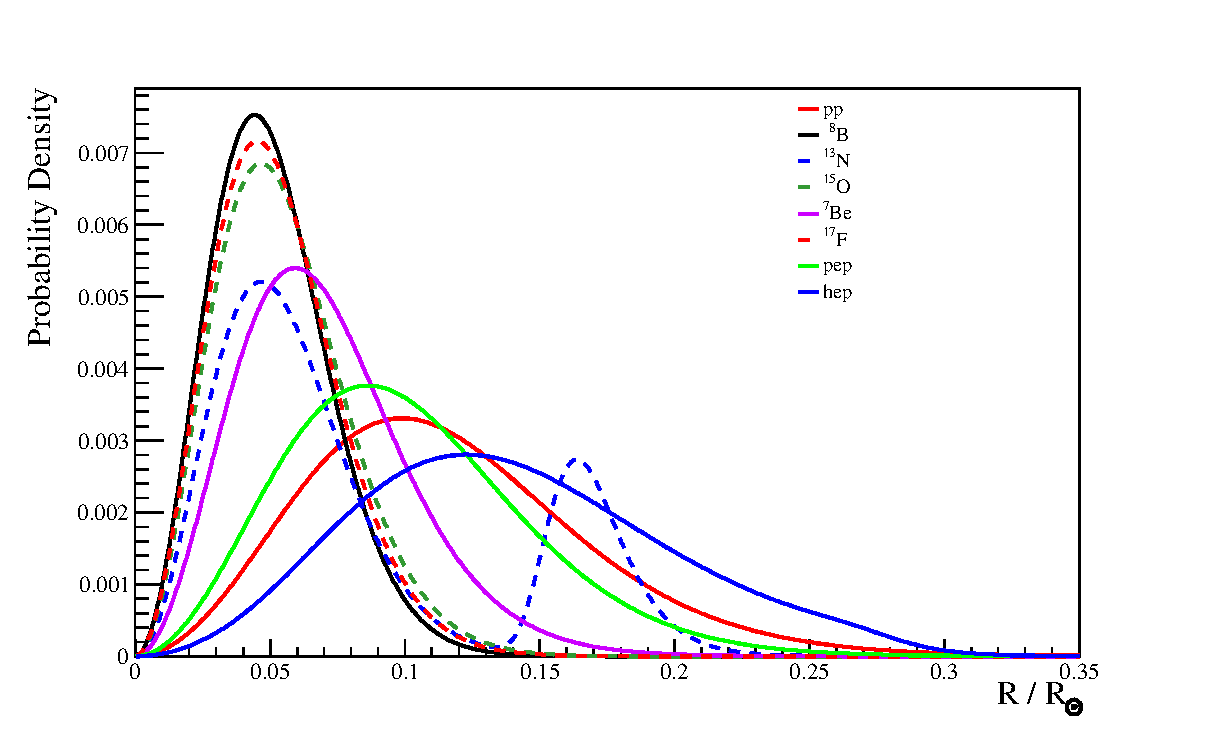
\includegraphics[width=0.8\textwidth]{solar_radial_production}
\caption[BS05OP Radial Production Profiles]{The radial
PDF for each solar neutrino production process. Values from BS05OP.}
\label{fig:radial_production_pdfs}
\end{figure}

\begin{figure}[htbp]
\centering
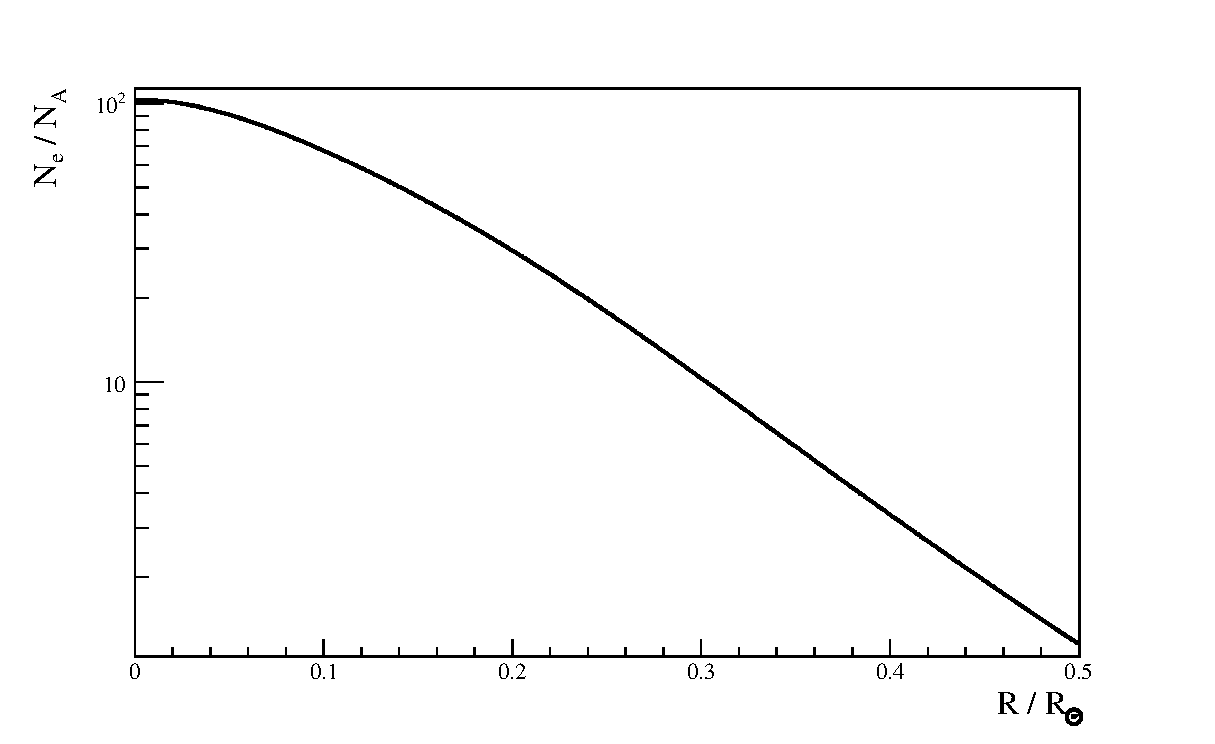
\includegraphics[width=0.74\textwidth]{solar_electron_density}
\caption[BS05OP Electron Density]{Electron density in units of Avogadro's
Number as function of radius in the Sun. Values from BS05OP.}
\label{fig:electron_density}
\end{figure}

Predictions for solar neutrinos rely heavily on solar modelling, which in turn
is constrained by helioseismological and photospheric measurements of the Sun.
Detailed solar models are used to simulate the evolution of the Sun from a proto-star
with a given mixture of chemical abundances and produce predictions for
what we would expect to observe today.
Following this procedure a temperature and density profile for the Sun can be determined
which in turn leads to predictions for solar neutrino production.
For this work the BS05OP~\citep{bs_ssm} solar model predictions are used.
Figure~\ref{fig:radial_production_pdfs} shows the solar neutrino production
distribution within the Sun.
Figure~\ref{fig:electron_density} shows the electron density profile within
the Sun.
The radial production distributions and electron density are necessary inputs
for solar neutrino mixing calculations.
%Photospheric and helioseismological measurements of chemical abundances provide input for solar models.

%and helioseismological measurements of the speed of sound in or across the Sun.  The speed of sound measurements can be used to estimate the require chemical composition.
%From this procedure the standard chemical abundances were determined~\citep{gs98}.
There are two standard estimates for the solar chemical abundances,
GS98~\citep{gs98} and AGS~\citep{ags}.
The BS05 model uses both as inputs and produces separate predictions for each,
in general this thesis uses the predictions from the GS98 abundances.
The most significant discrepancy between the two models is in the value
for the solar metallicity, the AGS prediction for the metallicity is
lower by roughly a factor of two.
The AGS estimates make use of a 3-dimensional model of the solar photosphere,
as opposed to the GS98 estimates which use a 1-dimensional model, however
the AGS model also produces discrepancies between photospheric measurements
and helioseismological measurements of the Sun~\citep{ags, bahcall01}.
The disagreements between the two models has become known as the
``Solar Metallicity Problem''.
%It's thought that solar neutrino measurements may be able 


\section{Solar Neutrino Mixing}
\label{sec:solar_nu_mixing}
Mixing for solar neutrinos is historically very important as it was
the measurements of solar neutrinos that provided the first evidence that
neutrinos mix at all~\citep{homestake,solar_nu_problem}.
Those measurements began the Solar Neutrino Problem, which wasn't solved
for nearly three decades and its eventual resolution by SNO and Super Kamiokande
led to the initial measurements of the neutrino mixing parameters~\citep{superk_atmospherics,
sno_second}.
Still today the Sun provides an unique source of neutrinos that travel through
densities and distances that cannot be produced by any other source, thus making
them a valuable object for study.
Chapter~\ref{sec:chameleons} discusses the study of mixing with
solar neutrinos further.

Neutrinos created in the solar core can experience significant matter enhanced mixing effects from local
electron density.
One of the most interesting aspects to neutrino mixing within the Sun is the MSW-effect,
at a specific electron density a resonance occurs and neutrinos are maximally mixed.
The condition for an MSW-resonance between any two matter states is given by
\begin{equation}
    N_{e} = \frac{\Delta m^{2} \cos2\theta}{2\sqrt{2}EG_{F}}\text{.}
\end{equation}
This condition is met for a 10\,MeV at an electron density
of $\frac{N_{e}}{N_{A}} \approx 20$ which occurs a solar radius of $0.25R_{\odot}$, 
for the mixing parameters given in~\citep{pdg_globalfit}.
For neutrinos with energy below approximately 5\,MeV this condition is not met
at any point within the sun, and so those neutrinos do not experience an MSW
resonance.
Once a neutrino created in the core of the sun has travelled past a solar radius of
approximately 0.5\,$\text{R}_{\odot}$ %TODO get a better number than this
the solar electron density has dropped far enough that matter effects are no longer significant
and neutrinos are effectively travelling through vacuum.% Once in the vacuum mixing dominated region

For solar neutrinos the neutrino states will generally evolve adiabatically from
matter effect dominated states to vacuum states.
However, when the neutrino transitions through the MSW-resonance
the flavor composition of the mass states changes rapidly,
which can lead to a non-adiabatic transition
between the mass-1 and mass-2 state.
For solar neutrinos the effect this transition has on the
neutrino survival probability is characterized with $P_{\mathrm{jump}}$,
\begin{equation}
    P_{\mathrm{jump}} = \mathrm{exp}\left[-\dfrac{\pi}{2} \dfrac{\sin^{2}2\theta_{12}}{\cos2\theta_{12}}
               \dfrac{\frac{\Delta m^{2}_{21}}{2E}}{\frac{1}{N} \frac{dN}{dx}|_{x_{R}}}   \right]
\text{\citep{parke}.}
\end{equation}
Where $x_{R}$ indicates the position at which the resonant density is crossed
and $N$ is electron density as a function of position.
For experimentally determined values of $\theta_{12}$ and $\Delta m^{2}_{21}$ in the so-called
Large Mixing Angle (LMA) regime the effect of $P_{\mathrm{jump}}$ is negligible.

\begin{figure}[htbp]
\centering
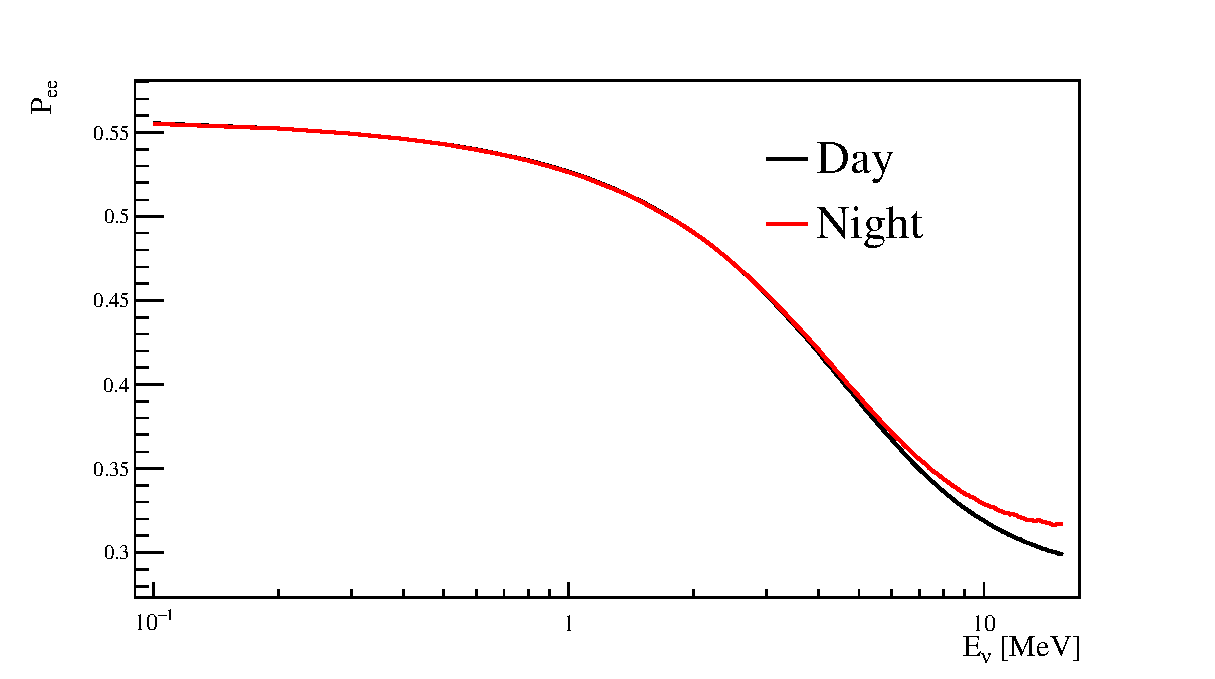
\includegraphics[width=0.84\textwidth]{day_night_example}
    \caption[Day and Night Survival Probability]{$\ce{^{8}B}$ survival
    probability during the day and night.}
\label{fig:day_night_example}
\end{figure}

One final feature of solar neutrino mixing is the ``day-night effect''.
The mantle, crust, and core of the Earth have sufficient electron density to provide
a non-negligible change to the effective neutrino mixing Hamiltonian.
Earth's atmosphere, however, is not dense enough to provide a significant
matter enhancement.
The relatively low density of the Earth's atmosphere, coupled with the fact that at higher energies neutrino mixing lengths
are $\mathcal(O)(100\mathrm{ km})$, means that neutrinos that travel a short
distance ($<\sim100$\,km) through the Earth will be detected in an
vacuum eigenstate.
Neutrinos that are travel a large distance in Earth's crust, mantle, or core,
will experience significant, potentially non-adiabatic matter effects, and will
be detected in a matter-enhance mass eigenstate.
For solar neutrinos the result is that neutrinos detected during the day, when
the Sun is directly above the detector, will not travel significantly through
the Earth;
neutrinos that are detected at night, when the detector is ``shadowed'' by the
Earth, will travel through large portions of the Earth.
Thus the effective survival probability is different during the day than the night.
Figure~\ref{fig:day_night_example} shows the survival probability during
the day and night.

\section{Neutrino Experiments}
\label{sec:experiments}
There's a long and diverse list of neutrino experiments that have contributed to
our current understanding of neutrinos, neutrino oscillations, and solar neutrinos.
I won't attempt to list them all here, but rather highlight the most immediately
relevant to this work;
These experiments play a significant role in the analysis described in Chapter~\ref{sec:chameleons}.
A more comprehensive review of neutrino experiments can be found in Ref.~\citep{giuntikim}.

%\subsection{Homestake}
%The first experiment to successfully detect solar neutrinos was the Homestake
%experiment.
%The detector was composed of approximately 100000 gallons of dry cleaning fluid.
%The choice of target was motivated by the high chlorine content in the cleaning
%fluid. Neutrinos above an energy of XXX would interact with the chlorine via
%beta decay, creating XXX. XXX would then decay to XXX with a half life of XXX.
%Periodically $\ce{^{3}He}$ was bubbled through the
%target liquid to extract the atoms of XXX that had been created. Once
%extracted those atoms were observed with proportional counters to count the
%number of XXX to XXX decays. The number of observed counts was proportional
%to the solar neutrino interaction rate, and therefore the solar neutrino flux.
%
%The Homestake experiment~\citep{homestake} ran from 1970 - 1990. %(XXX? is that right??)
%The experiment was able to provide the first measurement of the solar neutrino
%flux above XXX MeV. In 19XX they first reported a measure flux of
%XXX, nearly a third of the expected rate which was XXX.
%This deficiency became known as the solar neutrino problem, and it
%was the first evidence for neutrino oscillation.
%The deficiency was present across the entire lifetime of the Homestake experiment,
%their final report flux was XXX.

\subsection{SNO}
\label{sec:sno}
The Sudbury Neutrino Observatory (SNO) is a water-Cherenkov detector located
roughly $2$\,km underground near Sudbury Ontario in Canada, it ran from
$1999$ to $2006$ and detected primarily $\ce{^{8}B}$ solar neutrinos.
SNO had the unique feature of
being able to detect neutrinos through three different interaction channels,
each channel had it's own sensitivity to different flavor neutrinos.
Combining measurements from each interaction channel allowed for a measurement of the $\ce{^{8}B}$
solar neutrino flux that was not dependent on the flavor composition of the
incoming neutrinos.
This was accomplished by using a heavy-water ($\ce{^{2}H_{2}O}$ a.k.a. $\ce{D_{2}O}$) target and
detecting interactions through the electron-neutrino elastic scattering,
as well as charged and neutral current nuclear interactions on the deuterium
nuclei.
These interaction are described generally in Sec.~\ref{sec:neutrino_interactions}.
The NC interaction on deuterium can break apart the neutron and proton
that comprises the nucleus, $\nu_{x} + d \rightarrow p + n + \nu_{x}$.
The free-neutron can then capture on another deuterium atom forming tritium ($\ce{^{3}H}$)
and emitting an $6.2$\,MeV gamma which can be detected;
this process has no neutrino flavor dependence.
The CC interaction $\nu_{e} + d \rightarrow p + p + e^{-}$
is detected by observing the Cherenkov cone of the electron and will only
occur for electron flavor neutrinos.
The ES interaction is similarly detected from the scattered electron,
but the electron direction has a strong correlation with solar direction,
allowing the rate of ES interactions to be determined separately from the
rate of CC interactions.
The ES interaction occurs for neutrinos of all flavors, but with an increased
cross-section for electron flavor neutrinos.

SNO ran in the three phases, each phase with a different target
designed to increase the detectors ability to observe neutrons from neutrino
interactions.
The first phase had a pure $\ce{D_{2}O}$ target.
 The second phase loaded salt ($\ce{NaCl}$) into the heavy-water to increase
the neutron capture efficiency through observations of neutron capture on
chlorine instead of deuterium.
In the third phase an array of $\ce{^{3}He}$ proportional counters were added
to the detector, to once again increase neutron detection efficiency~\citep{sno_review}.

Some of the main results of the SNO experiment are summarized in
Figures~\ref{fig:sno_cross_graph} and~\ref{fig:sno_pee1}.
Their combined 3-phase result for the $\ce{^{8}B}$ flux is
\begin{figure}
\centering
\begin{subfigure}[b]{0.48\textwidth}
\centering
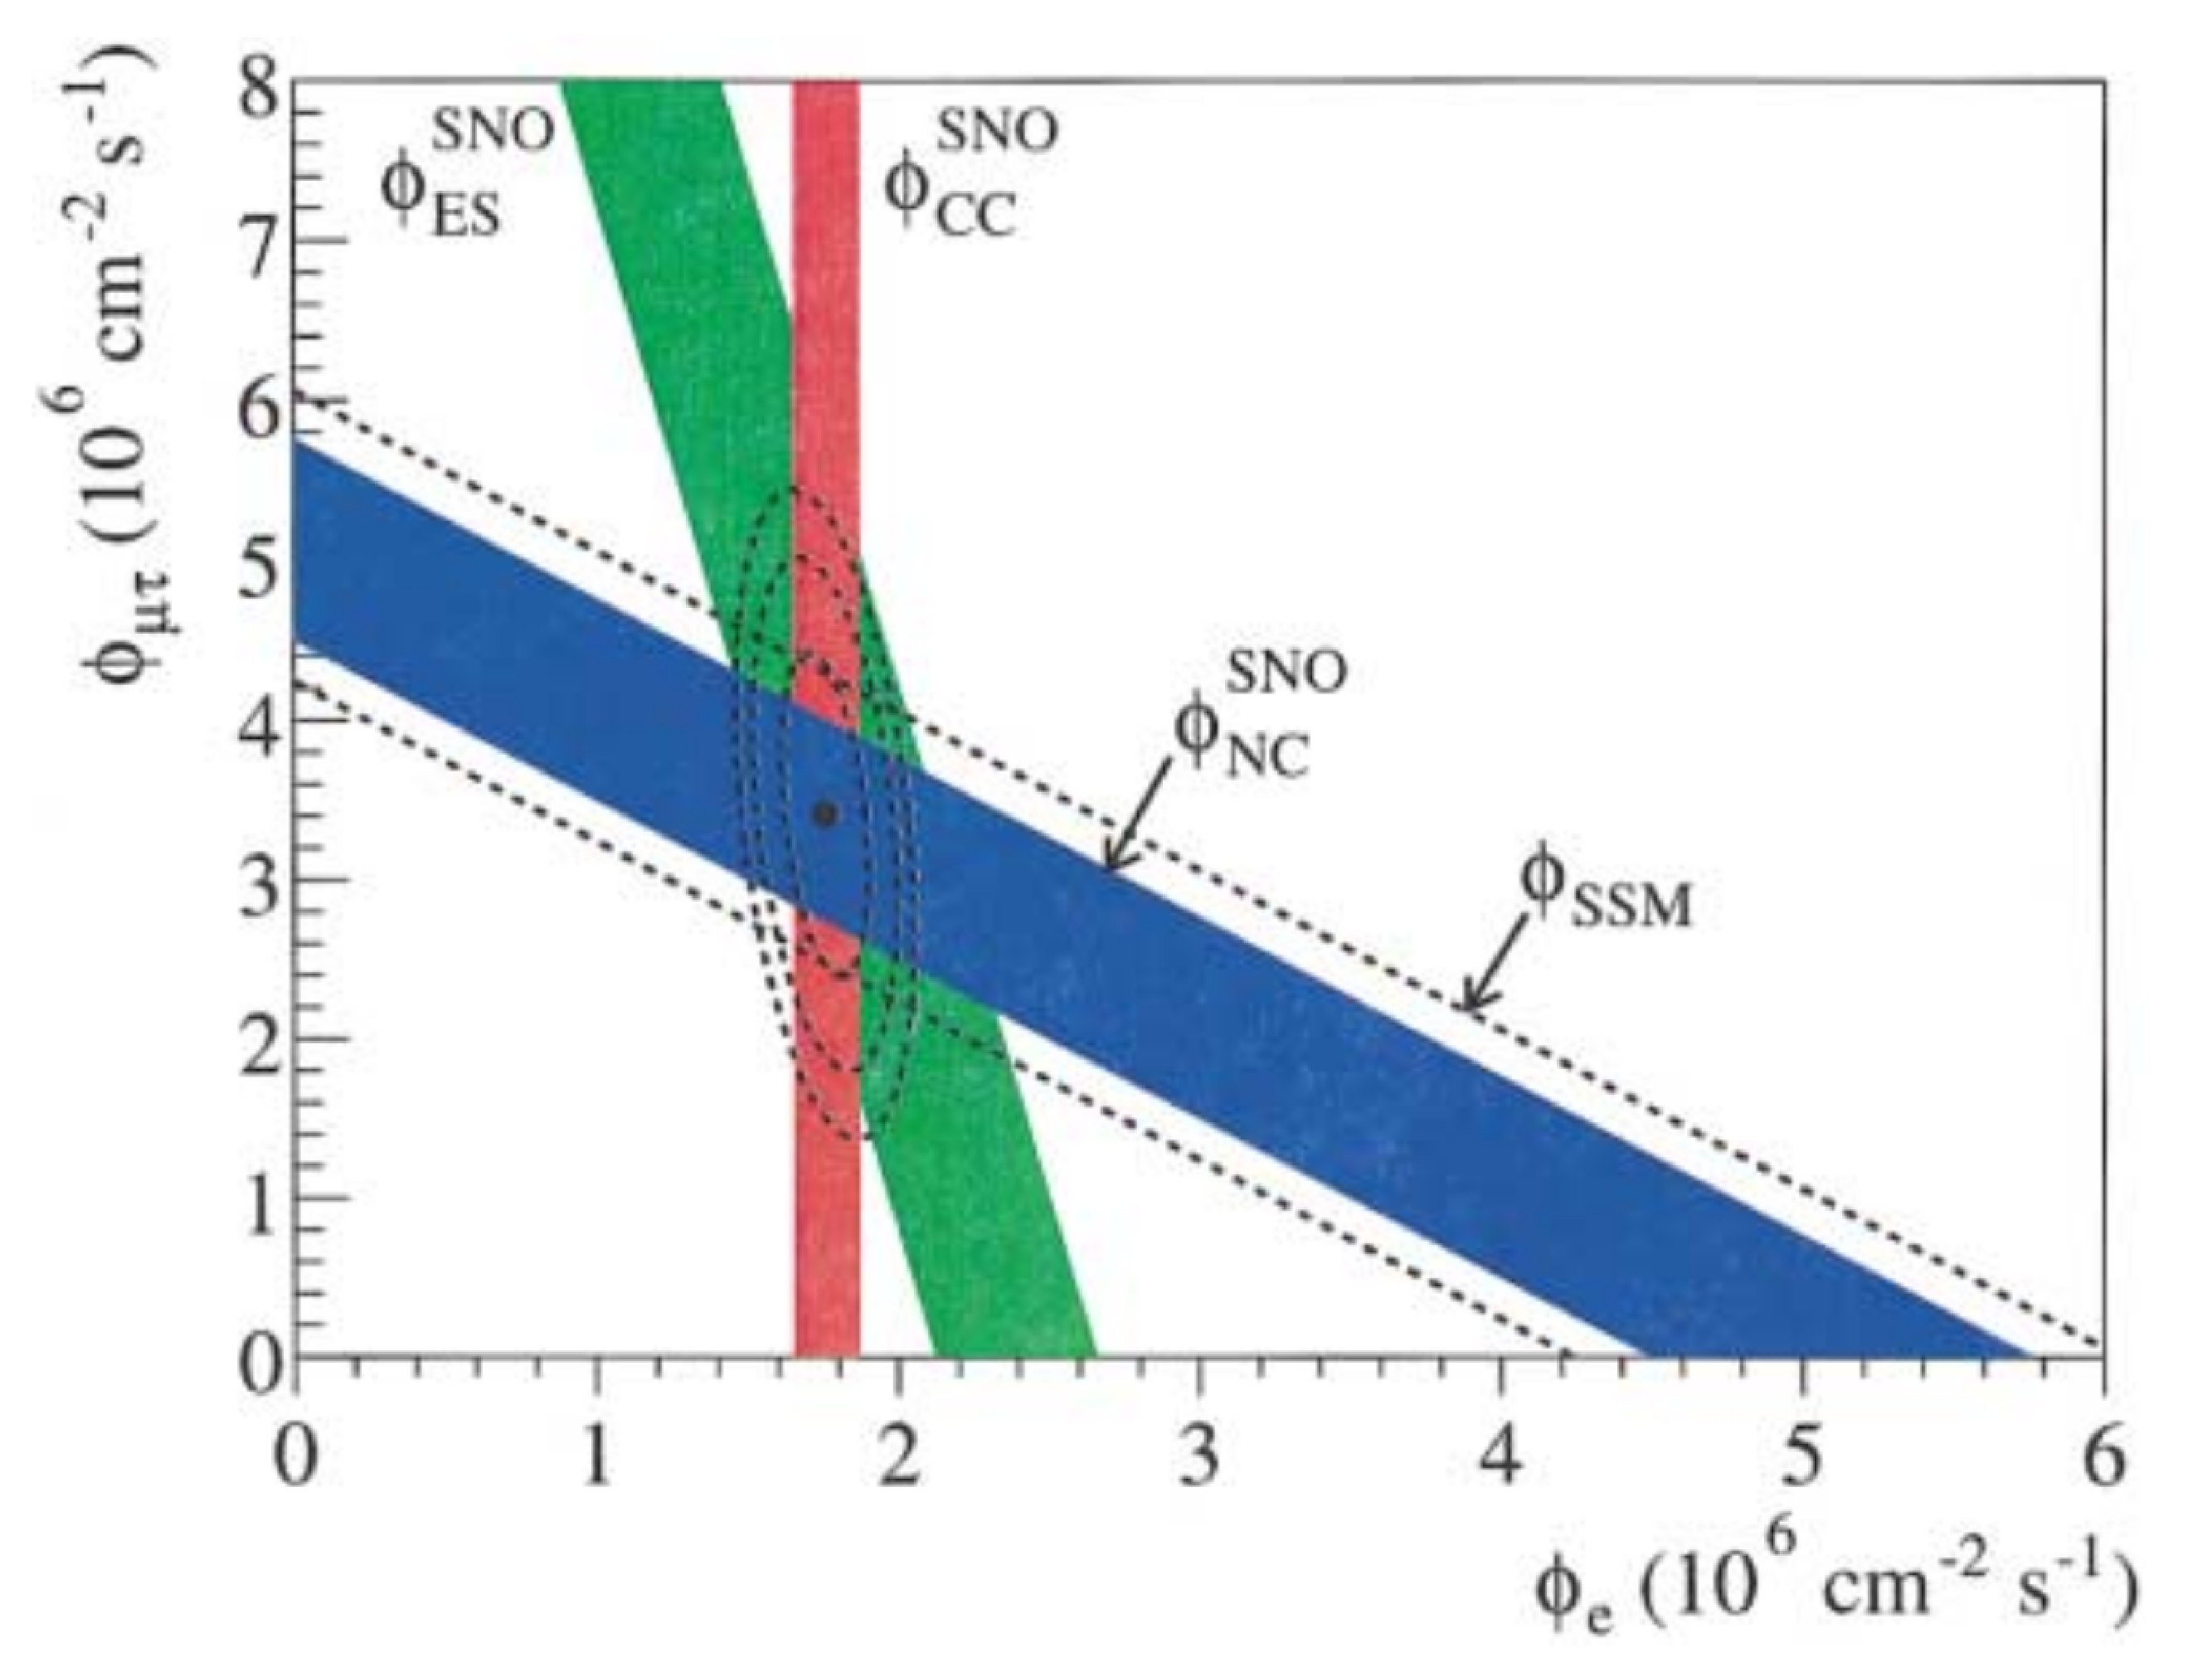
\includegraphics[width=\textwidth]{sno_cross_graph}
\caption[]{}
\label{fig:sno_cross_graph}
\end{subfigure}
\hfill
\begin{subfigure}[b]{0.48\textwidth}
\centering
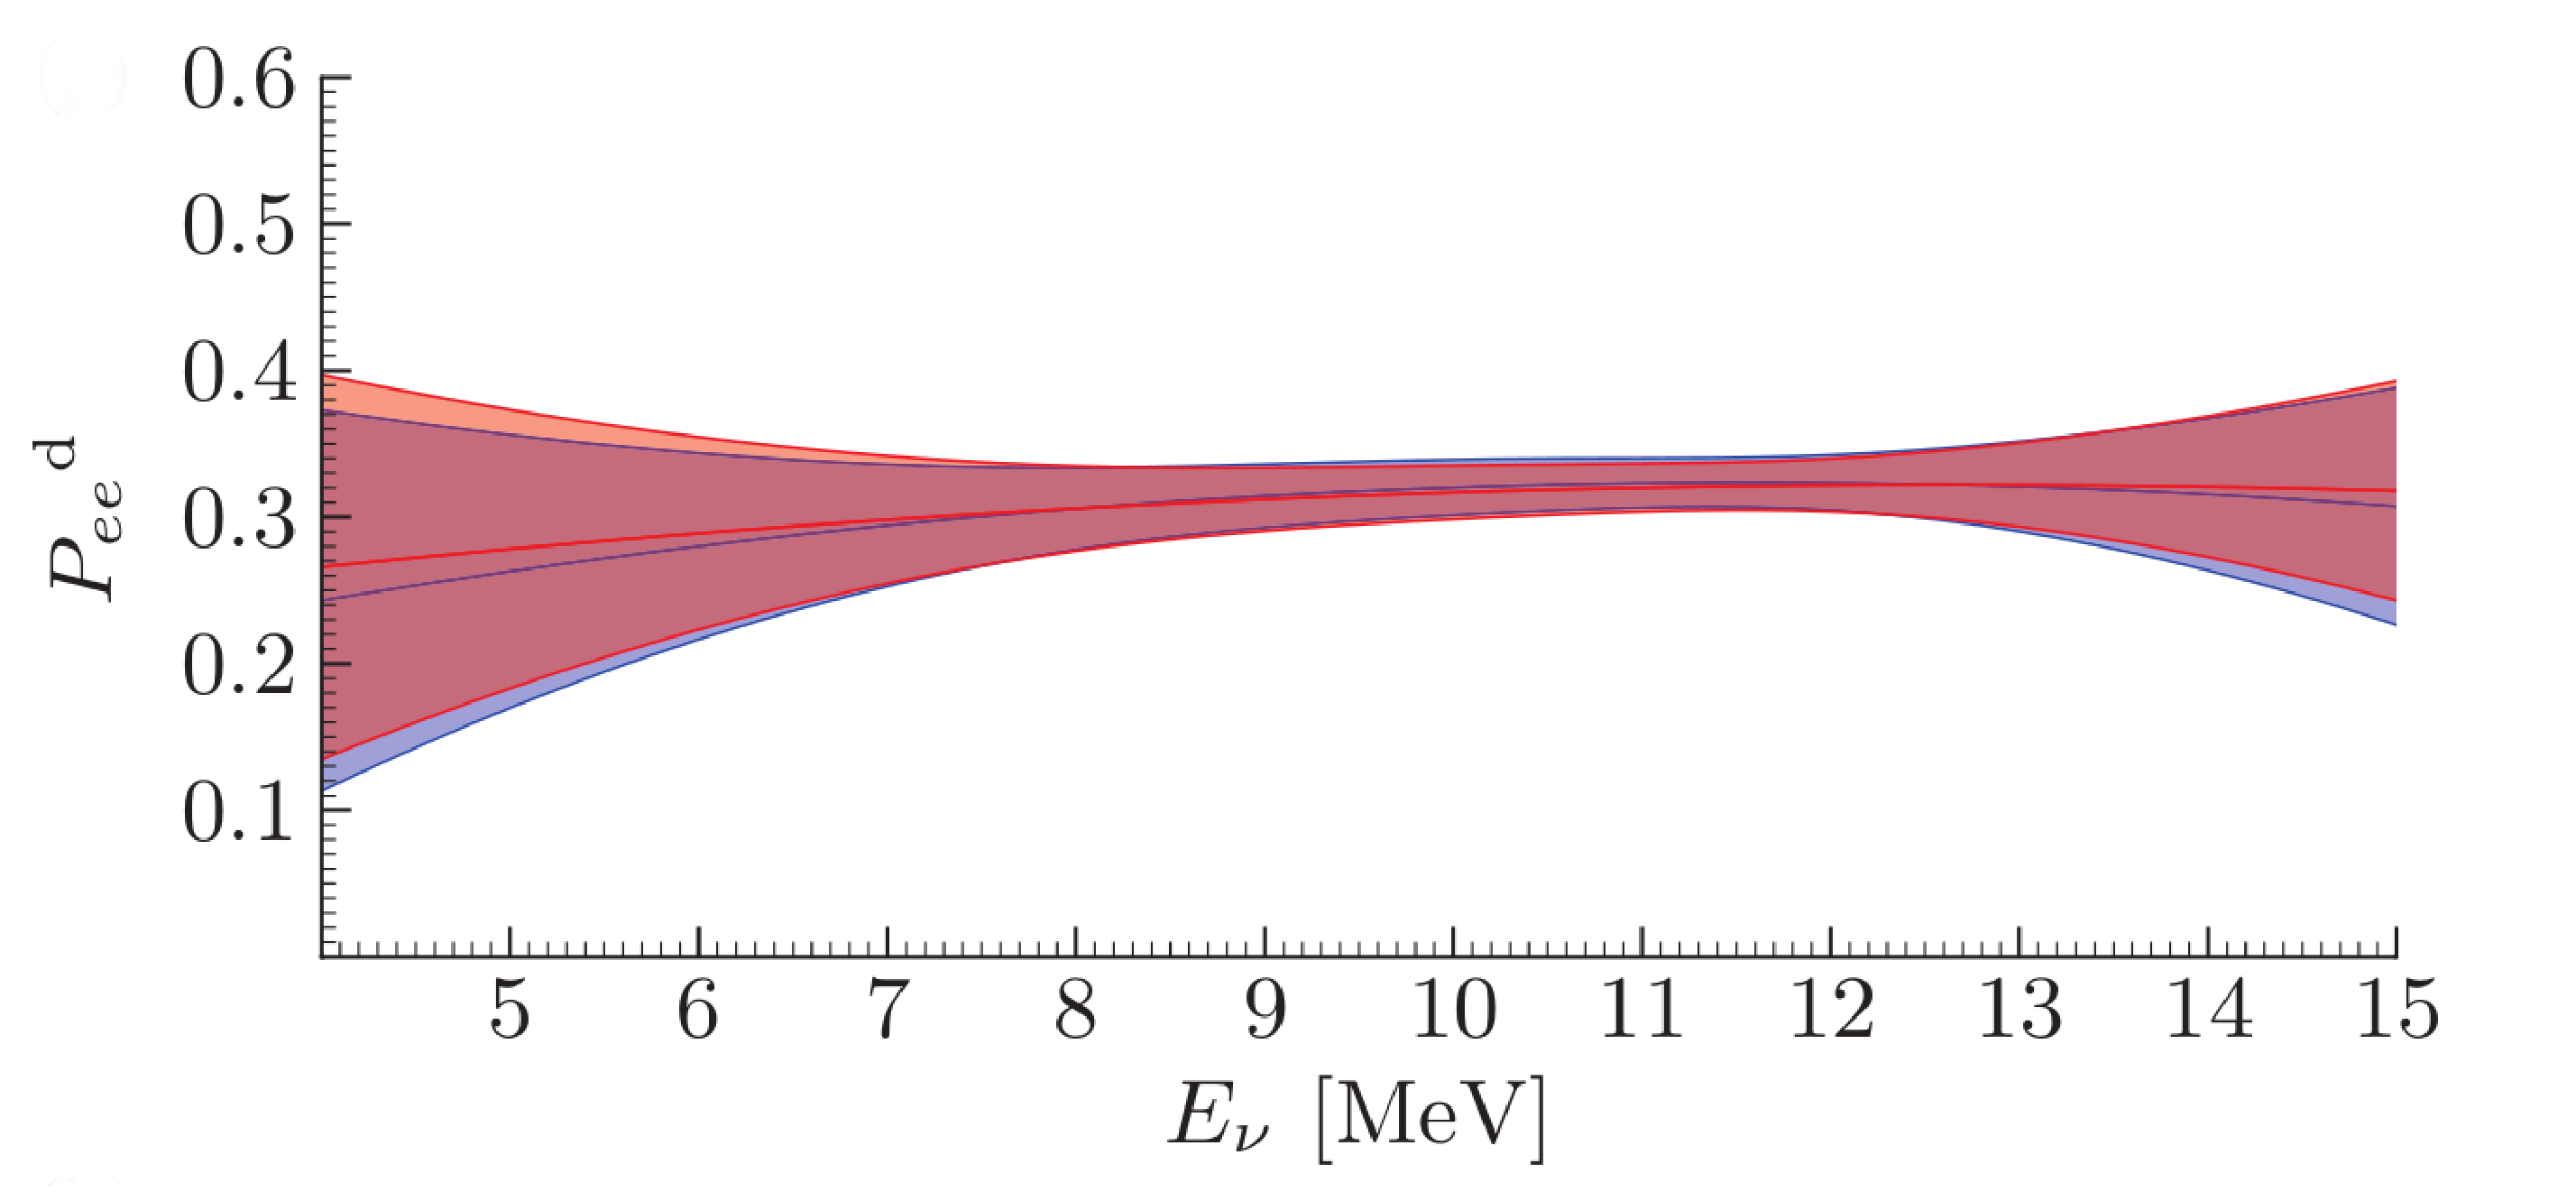
\includegraphics[width=\textwidth]{sno_pee}
\caption[]{}
\label{fig:sno_pee1}

\end{subfigure}
\caption[SNO Results]{(a) The extracted ES, CC, and NC rates in the
SNO experiment and how they relate to the
effective $\nu_{e}$ flux and $\nu_{\mu,\tau}$ flux; figure from~\citep{sno_second}.
 (b) The combined best fit survival probability from the combined three phase SNO
analysis (Ref.~\citep{sno_combined}), the red band is the best fit and uncertainty
from a maximum likelihood fit, the blue from a Bayesian fit.}
\end{figure}

\begin{equation*}
\Phi_{\ce{^{8}B}} = (5.25\pm0.16(stat.)^{+0.11}_{-0.13}(syst.))\times10^6\mathrm{cm}^{-2}\mathrm{s}^{-1}\text{.}
\end{equation*}
Their best fit mixing parameter estimates measurements are
\begin{equation}
\Delta m^{2}_{21}=(5.13^{+1.49}_{-0.98})\times10^{-5}\mathrm{eV}^2
\end{equation}
\begin{equation}
\tan^{2}\theta_{12} = 0.436^{+0.048}_{-0.036}\text{.}
\end{equation}
Values from Ref.~\citep{sno_combined}.

\subsection{Super Kamiokande}
Super Kamiokande (Super-K) is a 50\,kton cylindrical water Cherenkov detector.
It started running in $1996$ and has since made the most precise measurements of
atmospheric neutrinos and $\ce{^{8}B}$ solar neutrinos~\citep{superk4,superk4_atm}.
It's the successor to the Kamiokande experiment, which was a significantly
smaller and had a higher energy threshold for event detection.
Super-K can detect $\ce{^{8}B}$ solar neutrinos through only neutrino-electron elastic scattering,
they do not use a $\ce{D_{2}O}$ target and so are not sensitive to the
nuclear interactions similar to that of SNO\@.
Their extremely large detector volume though provides them extraordinary
statistics with which they've produced the most precise measurement of the $\ce{^{8}B}$
elastic scattering rate,
\begin{equation*}
\Phi_{\mathrm{ES}} = (2.308\pm0.020(stat.)^{+0.039}_{-0.040}(syst).)\times10^{6}\mathrm{cm}^{-2}\mathrm{s}^{-1}
\end{equation*}
Constraining the full $\ce{^{8}B}$ flux to the SNO result they've measured
the solar mixing parameters as,
\begin{equation*}
  \Delta m^{2}_{21} = 4.8^{+1.5}_{-0.8}\times10^{-5}\mathrm{eV}^{2}
\end{equation*}
\begin{equation*}
\sin^{2}\theta_{12} = 0.334^{+0.027}_{-0.023}\text{\citep{superk4}.}
\end{equation*}

\subsection{Borexino}
Borexino is 300\,ton spherical liquid scintillator detector~\citep{borexino_tdr}. Their detector
apparatus is similar to that of a water Cherenkov detector, the significant difference
is that the water is replaced with pseudocumene, a liquid scintillator.
A charged particle moving through scintillator generates roughly 50-100 times
more light than is produced by Cherenkov radiation alone.
Water-Cherenkov detector are typically limited in energy threshold
and energy resolution by the number of photons produced and detected, a liquid scintillator
detector solves this problem.  Scintillation light, unlike Cherenkov light,
is isotropic and provides no information about the direction the particle
was moving in.
\begin{figure}[htbp]
    \centering
    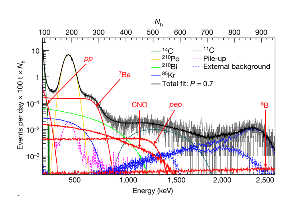
\includegraphics[width=0.75\textwidth]{borexino_spectrum}
    \caption[Borexino Spectrum] {Borexino's observed distribution of event energies with best fit
    signal and background model.
    $N_{h}$ is the number of prompt PMT hits.  Figure from~\citep{borexino_nature}.} %XXX Look up N_h to be sure
\label{fig:borexino_spectrum}
\end{figure}
\begin{figure}[htbp]
    \centering
    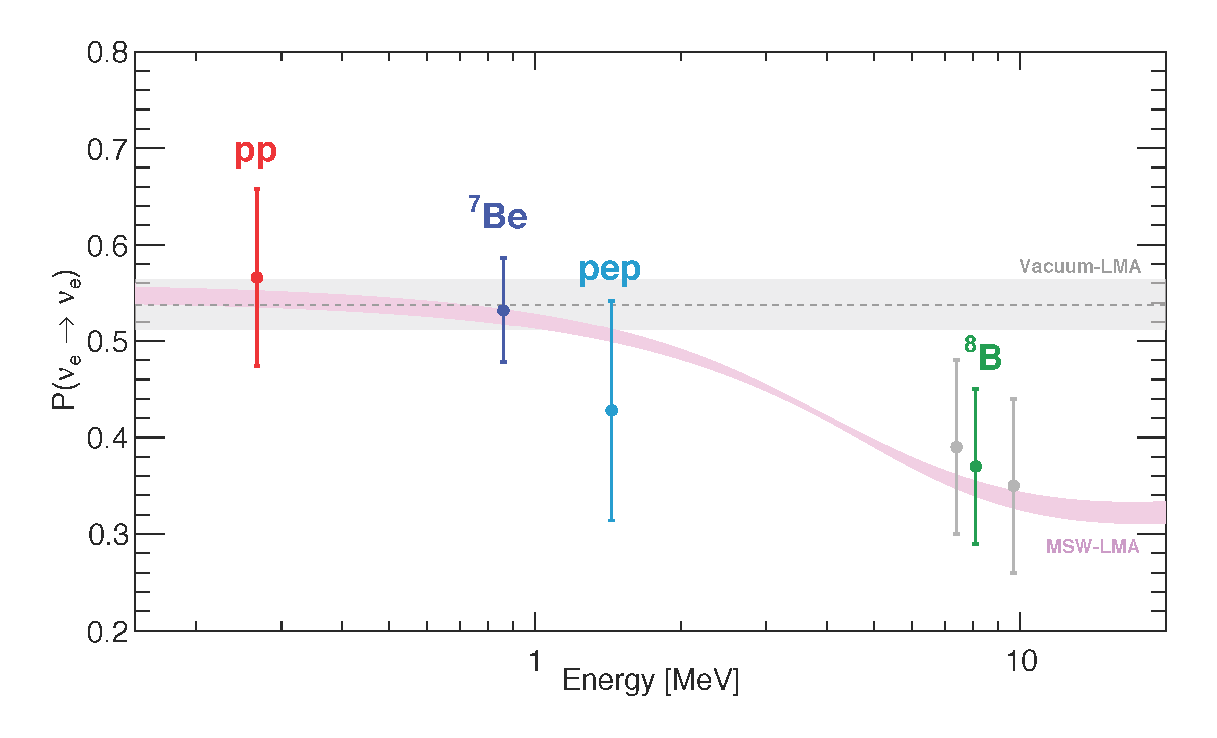
\includegraphics[width=0.75\textwidth]{borexino_pee}
    \caption[Borexino Survival Probability] {The best fit survival probability
    as measured by Borexino compared to the MSW modified neutrino mixing
    and vacuum only mixing. Figure from~\citep{borexino_nature}.}
\label{fig:borexino_pee}
\end{figure}

Water-Cherenkov detector are able to measure solar neutrinos by correlating the
direction of detected events with the position of the sun. Since Borexino is not
able to determine the direction of events within their detector, they instead
perform a spectroscopic measurement. The measurement requires
all sources of backgrounds to be accounted for and constrained from \textit{ex-situ}
measurements. Figure\ref{fig:borexino_spectrum} shows the observed spectrum by Borexino and the
spectra of the constituent solar fluxes and backgrounds.

Borexino took data from 2007 to 2016, with a pause in 2010 to remove source
of radioactive backgrounds and improve the radio-purity of their detector.
With that data they've measured $\ce{^{7}Be}$, $\ce{pep}$, $\ce{pp}$, and $\ce{^{8}B}$ neutrino
fluxes; they've also placed upper limits on the flux
of neutrinos from the CNO cycle and from the $hep$ solar reaction.
They're currently the only experiment to have measured the $\ce{pp}$ and $\ce{pep}$ neutrino
fluxes.
Figure~\ref{fig:borexino_pee} shows these results as the best fit survival probability
for each measured flux.

%$XXX$ FIND TABLE\\
%show spectrum and table of results

\subsection{KamLAND}
\label{sec:kamland}
The Kamioka Liquid Scintillator Anti-neutrino Detector (KamLAND) is a liquid-scintillator detector.
Its primary physics goals were the detection of reactor anti-neutrinos via
inverse beta-decay.
In addition to reactor anti-neutrinos KamLAND is also sensitive to solar neutrinos.
Performing a fit to the observed energy spectrum they were able to measure
the flux of $\ce{^{7}Be}$ and $\ce{^{8}B}$ solar neutrinos.
The $\ce{^{8}B}$ flux is reported as the ``elastic-scattering'' flux $\Phi_{ES}$, the flux of
pure electron flavor neutrinos that would produce the observed event rate.
They measure 
\begin{equation*}
\Phi_{ES\mathrm{,}\ce{^{8}B}} = 2.77 \pm 0.26(\mathrm{stat.}) \pm 0.32(\mathrm{syst.}) \times 10^6 \mathrm{cm}^{-2}\mathrm{s}^{-1}\text{\citep{kamland_b8}}.
\end{equation*}
KamLAND's reported $\ce{^{7}Be}$ flux, accounting for oscillation effects,  is
\begin{equation*}
\Phi_{\ce{^{7}Be}} = (5.82\pm 1.02)\times10^{9} \mathrm{cm}^{-2}\mathrm{s}^{-1}\text{\citep{kamland_be7}.}
\end{equation*}

\begin{figure}[htbp]
\centering
\begin{subfigure}[b]{0.75\textwidth}
\centering
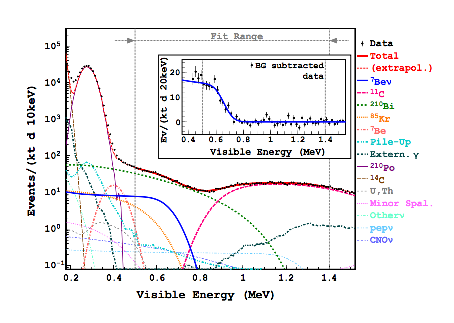
\includegraphics[width=\textwidth]{kamland_be7_spectrum}
\caption{}
\label{fig:kamland_be7}
\end{subfigure}

\begin{subfigure}[b]{0.75\textwidth}
\centering
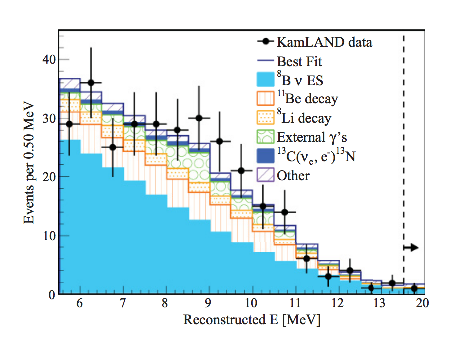
\includegraphics[width=\textwidth]{kamland_b8_spectrum}
\caption{}
\label{fig:kamland_b8}
\end{subfigure}
\caption{The observed reconstructed event energy spectrum for the Kamland Be7 flux measurement (a)
  and the 8B flux measurement (b). Figures from~\citep{kamland_be7} and~\citep{kamland_b8}.}
\label{fig:kamland_spectrum}
\end{figure}

Interestingly, KamLAND's reactor neutrino measurements~\citep{kamland_reactor} are
more relevant to the study of solar neutrinos than their solar neutrino measurements.
The long baseline (\urltilde180\,km) and low energy (\urltilde3\,MeV) of reactor neutrinos provides
unique sensitivity to $\Delta m^{2}_{21}$.
Other reactor neutrino experiments, such as Daya Bay, RENO, \& Double Chooz,
are primarily sensitive to neutrinos with too short a baseline to be strongly
affected by $\Delta m^{2}_{21}$.

\begin{figure}[htbp]
  \centering
  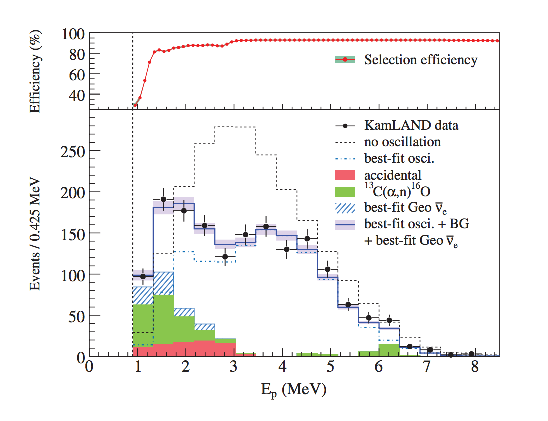
\includegraphics[width=0.75\textwidth]{kamland_reactor_spectrum}
  \caption[Kamland Reactor Spectrum]{Reactor anti-neutrino energy spectrum observed by KamLAND.
                                    Figure from~\citep{kamland_reactor}.}
  \label{fig:kamland_reactor}
\end{figure}

Figure~\ref{fig:kamland_reactor} shows reactor anti-neutrino energy spectrum measured
by the KamLAND experiment, with the best fit mixing parameters compared to the
expected spectrum with no oscillations.
From this measurement a best fit value of 
\begin{equation*}
    \Delta m^{2}_{21} = (7.58^{+0.14}_{-0.13}(\mathrm{stat.})^{+0.15}_{-0.15}(\mathrm{syst.}) )\times 10^{-5}\text{eV}^{2}
\end{equation*}
and,
\begin{equation*}
\tan^{2} \theta_{12} = 0.56^{+0.10}_{-0.07}(\mathrm{stat.})^{+0.10}_{-0.06}(\mathrm{syst.})
\end{equation*}
was determined.

The value for $\Delta m^{2}_{21}$ measured by KamLAND is in disagreement with
the value determined by solar experiments, although it cannot be ruled out that
the disagreement is a result of a statistical fluctuation. This discrepancy
will be discussed further in Sec.~\ref{sec:chameleons}.
